%% ----------------------------------------------------------------
%% Hardware Development.tex
%% ---------------------------------------------------------------- 
\chapter{Hardware and Firmware Development} \label{Chapter:HardwareDevelopment}
For initial development, the \textit{`Il Matto'} board, designed by Steve Gunn, was used. The system has an ATMega644P, 12MHz clock and an on board SD card socket. This provided the ability to prototype circuits which were then used to create a PCB.

This section is broken down into the following parts:
\begin{enumerate}
\item[\ref{Section:Camera}] Camera Code
\item[\ref{sect:SDCard}] SD Card
%\item Motor Control
\item[\ref{Section:Motor_Dev}] Motor Development
\item[\ref{Section:PCB_Dev}] PCB Development
\end{enumerate}

\section{Camera} \label{Section:Camera}

The camera used is an OV7670 by OmniVision. It is mounted onto a break out board and connected to a AL422B FIFO Buffer. The breakout board has all passive components and a 24MHz clock mounted. The schematic for the device can be seen in appendix \ref{Chapter:AppendixA:CircuitDiagrams}. The camera has a small hardware modification, due to a PCB fault. Pin 8 of the buffer is lifted and connected to pin 6 of the header, which is disconnected from the PCB (see figure \ref{fig:OV7670:Mod}).
\begin{figure}
\centering
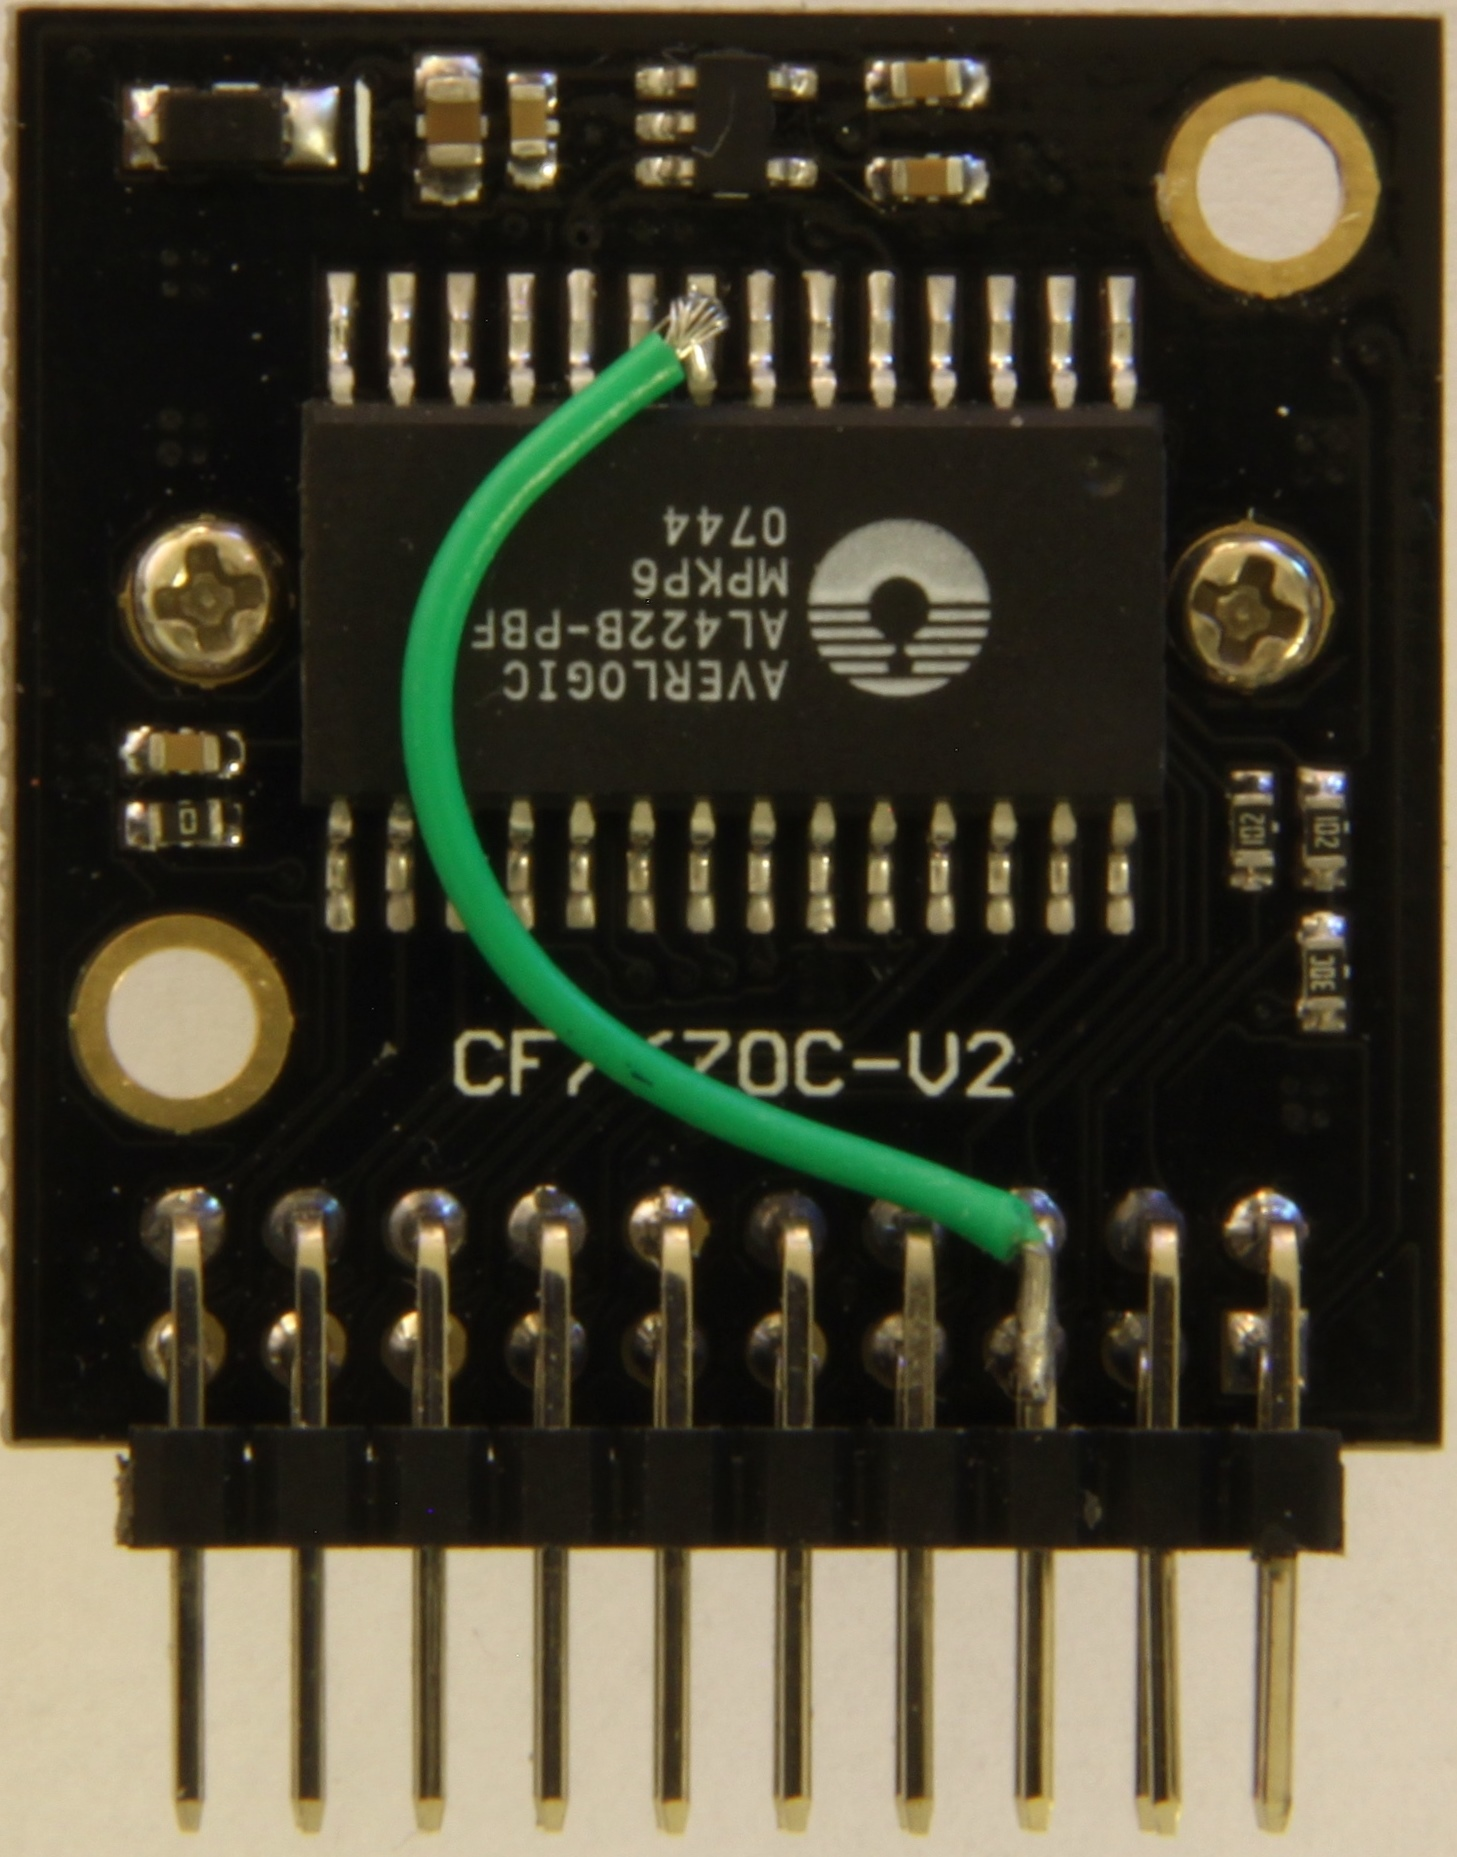
\includegraphics[width=\textwidth /4]{Figures/OV7670_Back.jpg}
\caption{Reverse side of the OV7670 Camera showing the modification}
\label{fig:OV7670:Mod}
\end{figure}
Original code for the camera operation was given by Steve Gunn which streamed continuous video to a TFT screen from the camera. The operation required was to take a single photo from the camera and store the data. 

\subsection{Single Camera Operation}

The camera uses a SCCB Interface \citep{SCCB_Interface} created by OmniVision. This is almost identical to the $I^{2}C$ Interface by Phillips and the two protocols are compatible. The original code for the camera used a software driven SCCB interface which was very slow and used up processing time. This was changed to make used of the built-in interrupt-driven $I^{2}C$ interface (named TWI in Atmel AVRs)\footnote{$I^{2}C$ , SCCB and TWI are all the same but are called differently due to Phillips owning the right to the name ``$I^{2}C$"}. This communication bus is used to write to the control registers of the camera to set up the signals, image format and image size. The set up procedure is used from the code given and sets the camera to function as explained below.

RGB565 is a 16 bit pixel representation where bits 0-4, 5-10 and 11-15, represent the blue, green and red intensity respectively (see figure \ref{fig:RGB565}). This is a compact way of storing data but only allows 65536 colours. Greys can also appear to be slightly green due to the inconsistent colour ratio of the green field. This representation was used as it is a compact format, easily converted to grey scale and is widely used.
\begin{figure}
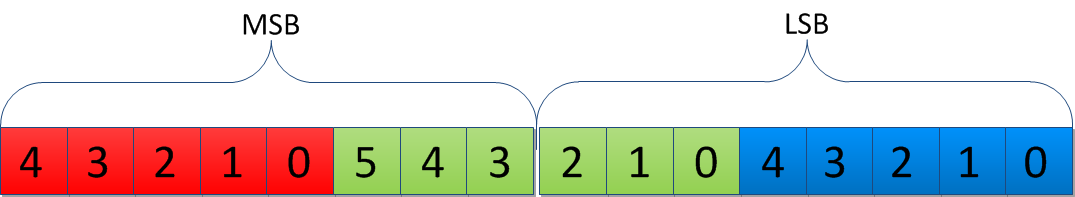
\includegraphics[width = \textwidth]{./Figures/RGB565.png}
\caption{RGB565 pixel format}
\label{fig:RGB565}
\end{figure}

The camera must use a high speed clock in order to ensure the pixels obtained are from the same time. This makes it difficult for an ATMega (typically clocked at 8-12MHz) to be able to respond to the camera quick enough. This highlights the necessity for a FIFO Buffer. 

The OV7670 is set up so that the VSYNC pin goes low at the beginning of every frame of data, and HREF is high when the data being output is valid. The pixel data is then clocked out on every rising edge of PCLK. To control the buffer, WEN (write enable) is NAND with the HREF signal. When both are high, the write enable to the buffer will be active and the data will be clocked in by PCLK. 

In order to acquire a full image, WEN must be high between two consecutive VSYNC pulses. VSYNC is set up to interrupt the AVR and a small state machine is implemented to count VSYNC pulses and control WEN correctly. After the WEN signal is pulsed, the buffer will contain all the valid pixel data.

To obtain the data from the buffer, the AVR sets output enable low and pulses the read clock. Valid data is available on the data port while RCLK is high. All the data is then read half a pixel at a time (the endianness of the data can be set up on the camera). 

After the data has been read, the buffer is reset by asserting the read and write reset signals (RRST and WRST) for at least one clock cycle of the relevant clock. The entire operation can be seen in figure \ref{fig:ov_Capture}.
\begin{figure}
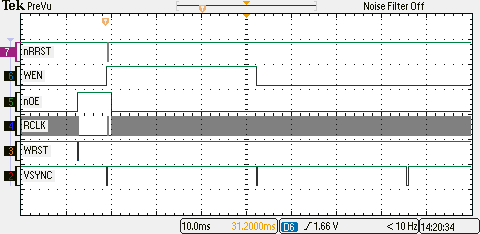
\includegraphics[width = \textwidth]{./Figures/ov7670_im_capture.png}
\caption{Signals generated to control the OV7670 capture and read}
\label{fig:ov_Capture}
\end{figure}


Difficulties arose at this point with the storage of the data. The ATMega644P has 4kB of internal SRAM, but  153.6kB of memory is needed to store a single image at QVGA (320 by 240 pixels, 2 bytes per pixel) quality. 

Firstly, data was sent to a desktop computer by USART. A simple program was written in C\# to receive and store all the data as a Bitmap image. This method was slow, taking around 30 seconds to transmit one uncompressed image. 

The second option was to use extra memory connected to the microcontroller. An SD card was used as FAT file system so the memory card is usable on a computer. Text log files were also written to aid debugging. This is discussed in section \ref{sect:SDCard}. 

\subsection{Dual Camera Operation}
In order for stereovision to be successful, two cameras separated by a horizontal distance ($B$) will need to be driven at the same time to obtain photos within a small time frame of one another.

A major problem occurred with using the \itc interface to set up both cameras. The camera has an \itc address of $21_{16}$, which cannot be changed. Multiple \itc devices with exactly the same address cannot be used on the same bus. 
Two solutions to this are possible: driving one from $I^{2}C$ and one from SCCB, or using an \itc multiplexer. By using two different buses the cameras will be individually addressable. However, SCCB is slow and processor-hungry as it is software driven. This takes up program memory and is not reusable for other operations.

An \itc multiplexer sits on one \itc bus and has multiple output buses. The master can then address the multiplexer and select whether to pass the bus to channel 0, channel 1 or not allow the data to be transferred. This saves processor time, but means a write operation has to be done to select the camera bus before being able to write to the camera. This slows down the operation slightly, but not as much as using SCCB. The main disadvantage to the \itc multiplexer is the extra hardware needed; firstly the multiplexer itself, but also 7 extra resistors to pull up the two extra buses and the three interrupt lines which aren't used, must be added. 

Overall, the disadvantages posed by using a multiplexer are small, so it was used as opposed to the SCCB interface. A suitable multiplexer is the Phillips PCA9542A \citep{I2C_Mux}.

The buffers have an output enable pin so the data bus can be shared by both cameras to the AVR. The ATMega644P offers three interrupt pins, two of which are used by the two VSYNC pins for the cameras to drive two individual ISRs. 

Operation to read an image is identical to using one camera. The code was duplicated so that the two cameras were accessed individually. Care was taken to avoid any bus contention on the data bus, but no checking is explicitly done. When taking a photo, both frames are taken at a time period close together to capture the same scenario. The data can then be read in either order and stored.

\section{SD Card} \label{sect:SDCard}

An SD card was chosen due to its small size, low cost and a large data storage. Smaller variants also exist, the mini and micro SD. The cards work using an SPI bus which can be used for other devices within the system as well. For the prototyping stage, the FATFS library \citep{FATFS} was used. This supplied all basic read and write operations for the SD card. For the AT32, the ASF supplied a more comprehensive FAT library and was used in the final product.

\subsection{Storing Images}

Many image formats are common, such as Joint Photographic Expert Group (JPEG), Portable Network Graphics (PNG), Bitmap (BMP) and Graphics Interchange Format (GIF). Table \ref{ImageFormats} shows a summary of these common image formats.


\begin{table}
\centering
\begin{tabular}{|p{3cm}| p{2cm}|p{2cm}|p{2cm}|p{2cm}|} \hline
			&	Bitmap 		& 	JPEG			 	&	PNG				& 	GIF \\ \hline
Extension 		& 	*.bmp 		&  	*.jpg /*.jpeg 		& 	*.png				& 	*.gif \\ \hline
Compression 	& 	No 			& 	Lossless  and Lossy		&	Lossless ZIP			&	Lossy	\\\hline
File Size of 320 by 
240 pixel Image (kB) &	225			&	20				&	23				&	24 \\\hline
Bits per Pixel		&	8, 16, 24 or 32	&	24				&	24, 32 or 48 			& 	24, but only 256 Colours \\


\hline
\end{tabular}
\caption{A table comparing different image formats available \citep{ImageComparison}}
\label{ImageFormats}
\end{table}

It is clear that the best choice for images would be either PNG or JPEG. However, these require more computational time to compress the image into the correct format. To avoid compression, and thereby save processing time, bitmap was chosen at the expense of using more memory. The data in a bitmap image is also stored in RGB format so can be read back easily when processing the image. Appendix \ref{Chapter:AppendixB:BMPFile} shows the make up of a Bitmap File that was used.

By writing the image in this format, they are then able to be opened on any operating system. This aids debugging and allows the prototyping of image algorithms in a more powerful environment. Figure \ref{ExampleImage} shows a photo taken by the OV7670 and stored on a SD card. The quality is not professional, but all features can be seen. The colour is accurate and large text can be read at a small distance. Though the images were able to be opened in most programs, MATLAB gave errors when reading the bitmaps. This could be avoided by opening and resaving the images in MS Paint.

\begin{figure}
\begin{center}
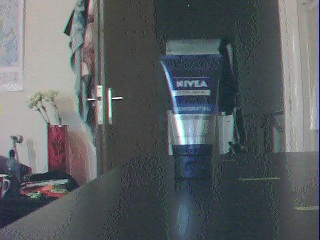
\includegraphics{Figures/ExampleImageFromCamera.jpg} 
\end{center}
\caption{An Example Image taken using the OV7670 and stored as a Bitmap on the SD Card}
\label{ExampleImage}
\end{figure}

\section{The Prototypes}

The first prototype made can be seen in figure \ref{fig:Prototype}. This obtained two images from both cameras, and stored them to the SD Card. The cameras shared the data bus and a \itc multiplexer was used. An ATMega168 was added to the system as no pins remained for debugging on the \textit{Il Matto} board. The pinout for the 644 can be seen in table \ref{table:644Pin}. The ATMega168 used the already existing \itc bus and acted as a port extender - button inputs were read and status LEDs were written to. This enabled a debug output for the system. The prototype worked well and proved the circuit worked. 

A second prototype was made to stream the images to a TFT screen. This can be seen in figure \ref{fig:Prototype:TFT}. This provided the ability to check the cameras worked, and gave a live stream so the lens could be focused to give a clear image. The refresh rate of a full image was slow ($\approx 0.6fps$), but the system was successful.w

\begin{table}
\centering
\begin{tabular}{|c|c|c|c|c|}\hline
	& 	Port A 	& 	Port B 			& 	Port C 				& 	Port D 		\\ \hline
0	&	Data 0	&	SD Write Protect&	\itc - SCL			&	No Connection	\\
1	&	Data 1	&	SD Card Detect	&	\itc - SDA			&	No Connection	\\
2	&	Data 2	&	USB Data Plus	&	Read Clock 1		&	VSync 0			\\
3	&	Data 3	&	USB Data Minus	&	Read Reset 1		&	VSync 1			\\
4	&	Data 4	&	SPI Chip Select	&	Write Enable 1		&	Read Clock 0	\\
5	&	Data 5	&	SPI	MOSI 		&	Write Reset 1		&	Read Reset 0	\\
6	&	Data 6	&	SPI MISO		&	Output Enable 0		&	Write Enable 0	\\
7	&	Data 7	&	SPI Clock		&	Output Enable 1		&	Write Reset 0	\\
\hline

\end{tabular}
\caption{Pin Connections of the ATMega644P for Dual Camera Operation.}
\label{table:644Pin}
\end{table}

\begin{figure}
\includegraphics[width=\textwidth]{./Figures/Prototype.jpg}
\caption{Prototype of Dual Camera operation.}
\label{fig:Prototype}
\end{figure}

\begin{figure}
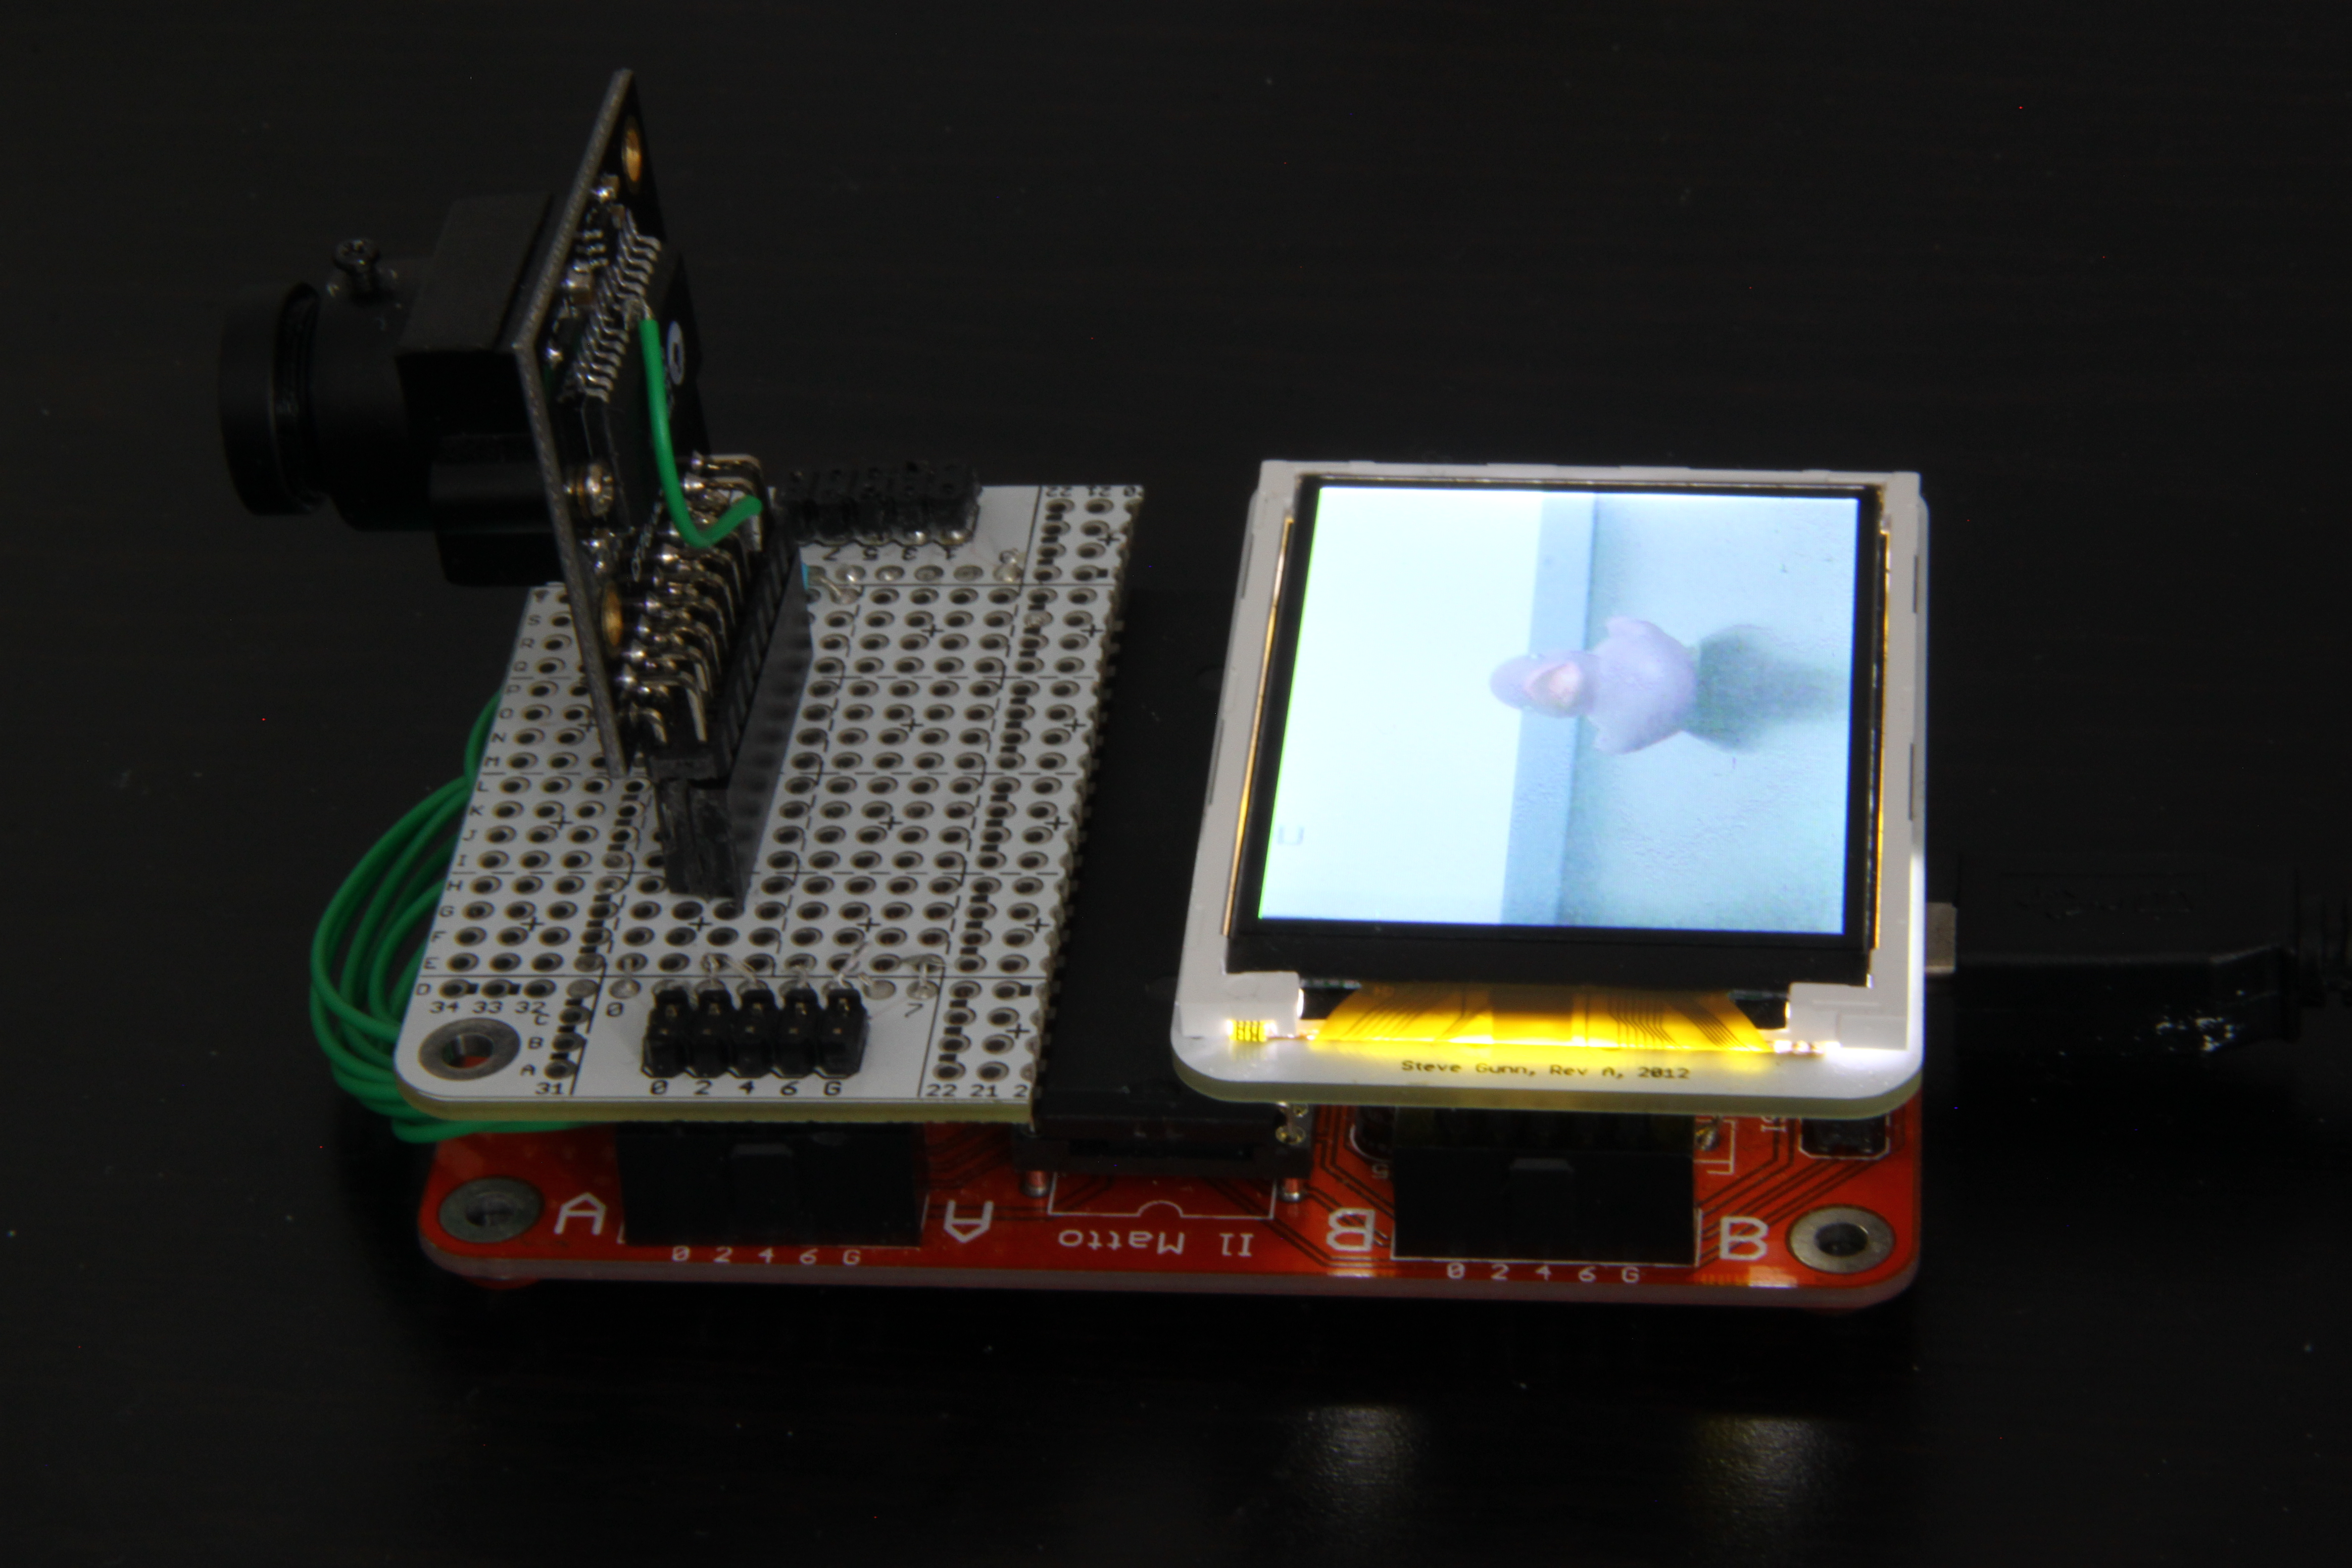
\includegraphics[width=\textwidth]{./Figures/Camera_TFT.jpg}
\caption{Prototype of streaming camera images to TFT screen.}
\label{fig:Prototype:TFT}
\end{figure}

\section{Motor Driver Development}\label{Section:Motor_Dev}
%\inote{Tachometers}
%\inote{Derivation of equations used - Distance / Rotating}

\subsection{Hardware}
Tachometers are devices used to measure rotational speed of a wheel. They are commonly found in bicycles where a small magnet is attached to the wheel and a sensor is attached to the frame. The elapsed time between every rotation is measured by the and speed can be calculated given the wheel size. 

Here an optosensor, the TCRT1010 made by \cite{Vishay:TCRT1010:Datasheet}, is used to measure rotations of the wheel and therefore be able to move a distance determined by the microcontroller. The TCRT1010 package contains an IR LED and a phototransistor. The schematic of a simple transistor amplifier used can be seen in figure \ref{Circuit:TCRT1010} which was reproduced from \cite{c9Lab:SRG}. 

A similar method to the way a bike measures speed was used. The wheel's rubber absorbed the IR from the LED, so a high voltage was always seen at the collector of the phototransistor when near the wheel. White Tipp-Ex marks, ``tabs'', were applied to the wheels at regular intervals. These tabs reflected IR, resulting in a lower collector voltage when aligned and thereby giving a way to detect wheel rotation. Figure \ref{Graph:WheelVoltage} shows the voltage at the collector (read by the ADC on the AVR) against the angle of the wheel. Ten tabs were marked on the wheel, and ten dips in the voltage can be seen in figure \ref{Graph:WheelVoltage}. A lot of noise exists due to imperfect white tabs. However, the dips are prominent and can be detected with the correct threshold voltage.

\begin{figure}
\centering
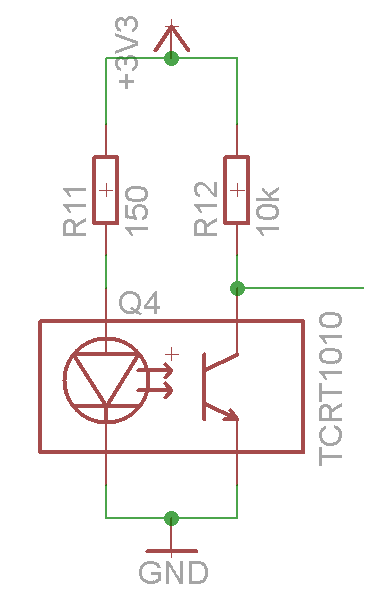
\includegraphics[scale=0.5]{Figures/TCRT_Circuit.png}
\caption{Circuit diagram of Optosensor}
\label{Circuit:TCRT1010}
\end{figure}

\begin{figure}
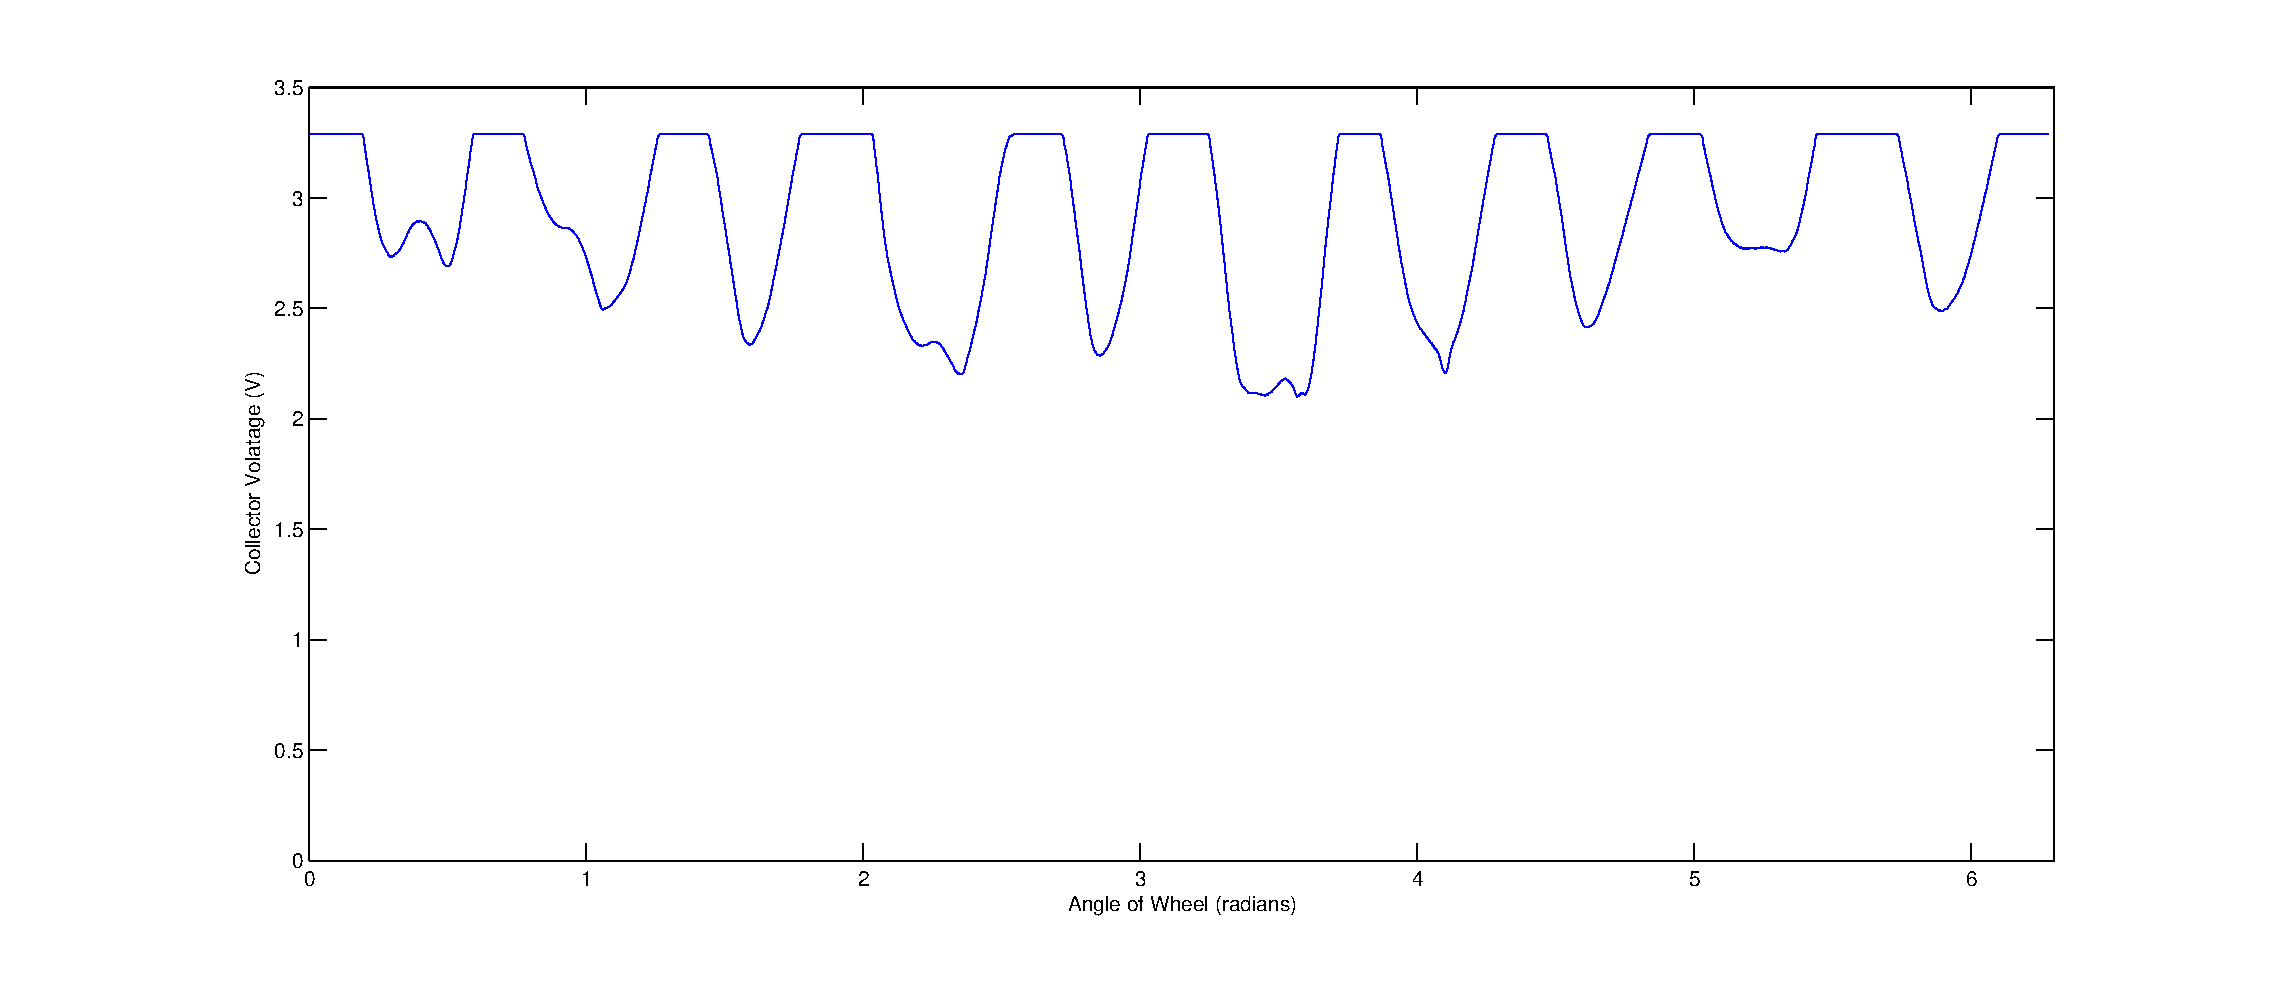
\includegraphics[width = \textwidth]{Figures/WheelVoltageGraph.eps}
\caption{Graph of Wheel Angle against the Voltage read by the AVR}
\label{Graph:WheelVoltage}
\end{figure}
 

\subsection{Firmware Development}

To move a distance, the number of times a tab passes the sensor, a count, must be detected. The firmware sets up a PWM output and has set up and execute functions. A low duty cycle PWM signal was used to drive the motors slowly. This removed the need for a speed controller and meant any overshoot of the motors during breaking would be low. Straight line movement and spot rotations were implemented. More complex movements, for example arcs, would require more accurate tachometers and are not discussed here. 

\subsubsection{Set Up}
The set up calculates the number of counts needed, and sets the direction of the wheels. Each motor driver has two inputs to control direction and table \ref{table:MotorDirection} shows the inputs needed to generate the two movements - straight line and rotational. 

\begin{table}
\centering
\caption{A table to show the inputs to the motor drivers to set the movement}
\label{table:MotorDirection}
\begin{tabular}{|c|c|c|c|c|c|c|}\cline{2-7}
\multicolumn{1}{c|}{ }&\multicolumn{3}{|c|}{Motor 1}&\multicolumn{3}{|c|}{Motor 2}\\\cline{2-7}
\multicolumn{1}{c|}{ }	&	STBY 	&	IN1	& IN2 	& STBY 	& IN1 	& IN2	\\ \hline
Stop					&	0		&	X	&	X	&	0	&	X	&	X	\\
Forward					&	1		&	1	&	0	&	1	&	1	&	0	\\	
Backward				&	1		&	0	&	1	&	1	&	0	&	1	\\
Clockwise				&	1		&	1	&	0	&	1	&	0	&	1	\\
Anti-clockwise 			&	1		&	0	&	1	&	1	&	1	&	0	\\\hline
\end{tabular}

\end{table}

To move in a straight line, the number of counts can be calculated by equation \eqref{eq:NumberCounts}. 

\begin{equation}
\label{eq:NumberCounts}
\text{Counts} = \delta \times \frac{\gamma}{C_w}
\end{equation}

For rotation, the radius from the centre of the robot to the wheels needs to be known, see figure \ref{fg:RobotBase:Top}. The circumference through the wheels is then easily calculated and the distance to move is calculated by equation \eqref{eq:RotationalDistance}. The total number of interrupts can be calculated using equation \eqref{eq:NumberCounts}. 

\begin{equation}
\label{eq:RotationalDistance}
\delta_{R} = A \times \frac{C_b}{360}
\end{equation}

Combining equations \eqref{eq:NumberCounts} and \eqref{eq:RotationalDistance} gives:
\begin{equation}
\label{eq:RotationalInterrupts}
Counts = \gamma \times \frac{C_b}{C_w} \times \frac{A}{360}
\end{equation}
Figure \ref{fig:RobotBase_Annotated} shows the dimensions of interest of the robot base. In the set up method, equations \eqref{eq:NumberCounts} and \eqref{eq:RotationalInterrupts} are used to calculate the counts needed. The results are placed in the global struct and the execute method is then run.

\subsubsection{Execute}

The execute method detects the tabs and decrements the global counter. When the counter reaches zero the motor stops and when both motors have completed, the method exits.

As the voltage swing on the collector of the phototransistor did not reach near 0V, the AVR could not detect this as a logical 0. An external amplifier could have been used to generate a full swing voltage. However, the AVR has internal ADCs and analogue comparators which were used instead. 

The ADC could be used to continually sample the collector voltage and detect dips in the signal. This method has the advantage of a variable threshold and the ability to filter noise. The operation, however, would be complex to implement in code. 

An alternative was to use an analogue comparator. The UC3C has two on chip comparator interfaces, each with two comparators. They are a high gain operational amplifier with added options of hysteresis and the ability to interrupt amongst other attributes. The comparators can use two analogue inputs or use the internal DACs as inputs. Potentiometers were used to set the reference voltage externally. Using the comparators had the advantage of returning a boolean value of if the collector voltage is higher or lower than the threshold voltage. The detection is of a tab was then simpler. This method was decided on for an easier implementation.

The first method implemented was to use the analogue comparators to interrupt when the collector voltage crossed the threshold. Both wheels used the same comparator interface and therefore ran the same ISR when triggered. The ISR then had to read the output of the comparators and decrement the relevant counter for the correct wheel. This method had many downfalls. First, it was not possible to know which comparator caused the interrupt. If the left wheel triggered the interrupt while the right was below the threshold, both left and right counters would be decremented. This caused a large error each time it occurred. Another problem was noise; occasionally, the lowering voltage would cause multiple interrupts each time. This problem was reduced by setting the hysteresis on the comparators but did not solve the problem completely. 

A second approach utilised a simple state machine and software based hysteresis to solve the problems. The state machine has two states `On a Tab' and `Not on a Tab'. When the method enters, the initial state is read from the comparators so that if the wheel is already on a tab, it won't be counted. The code then runs in a loop until the motors stop. A graphic representation of the code can be seen in figure \ref{fig:StateMachine}. Starting in `Not on a Tab' state, a tab must be detected for Hyst\_Max amount of cycles in succession for the state to change. This is the same for going from `On a Tab' to `Not on a Tab'. This is to reduce noise in the form of false readings an increase the certainty that a tab is in detect. The Global\_Count is only reduced on the transition to `On a Tab' so it is difficult for this to decrement multiple times in normal operation. To increase the certainty, Hyst\_Max can be increased at the expense of response time. 


\begin{figure}
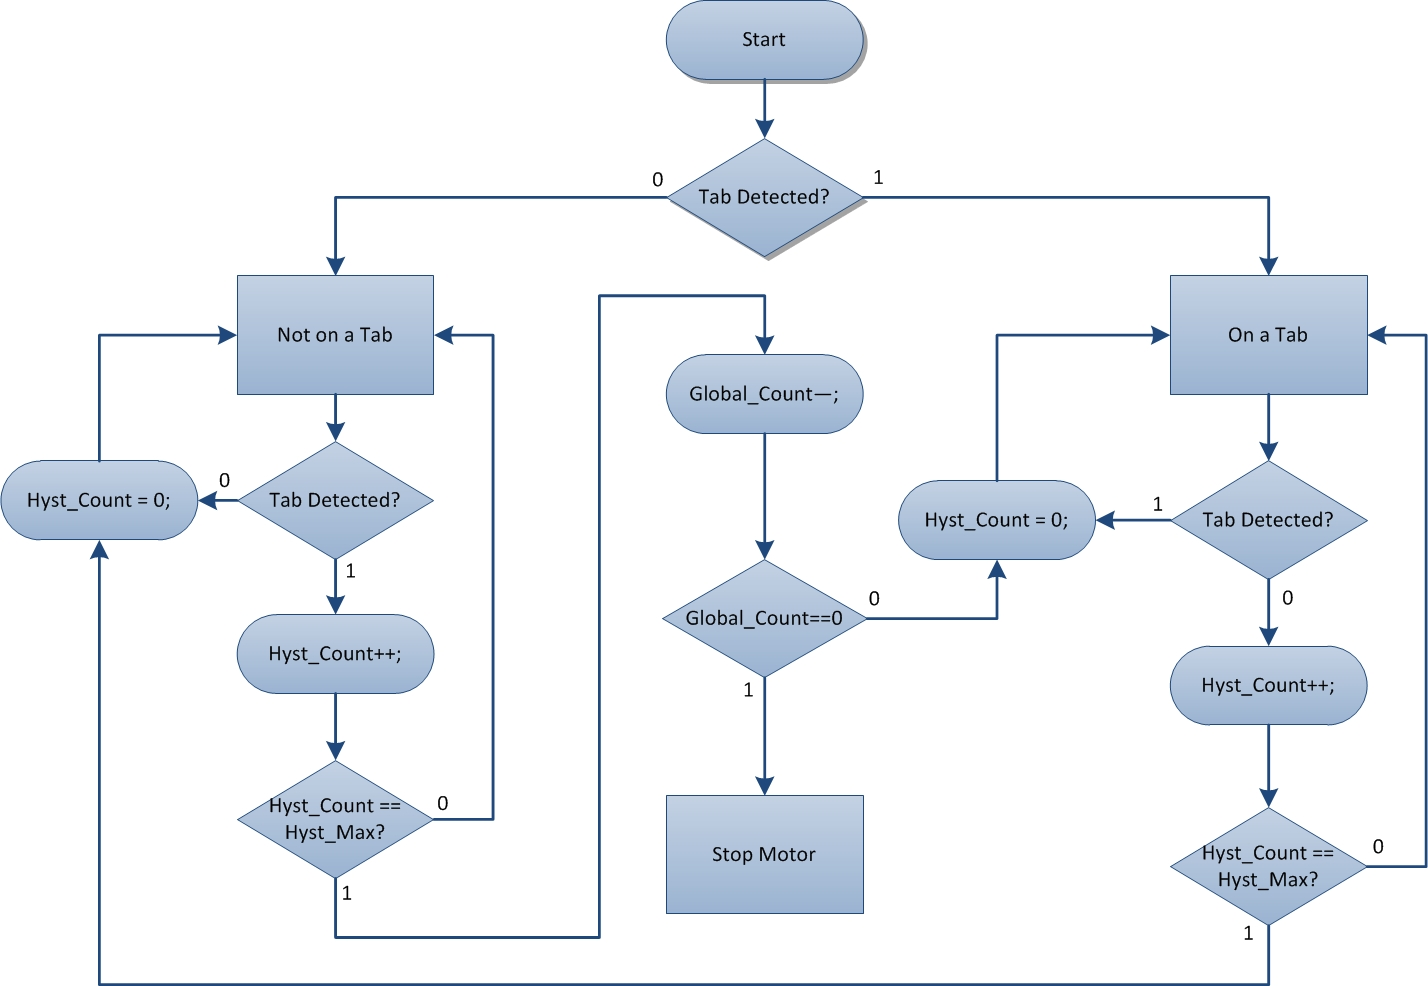
\includegraphics[width=\textwidth]{Figures/ASM.jpg}
\caption{A State Machine showing the operation of the \textit{Motor\_Execute} method}
\label{fig:StateMachine}
\end{figure}


\begin{figure}
\centering
\subfigure[Top View of robot base showing dimensions of interest\label{fg:RobotBase:Top}]{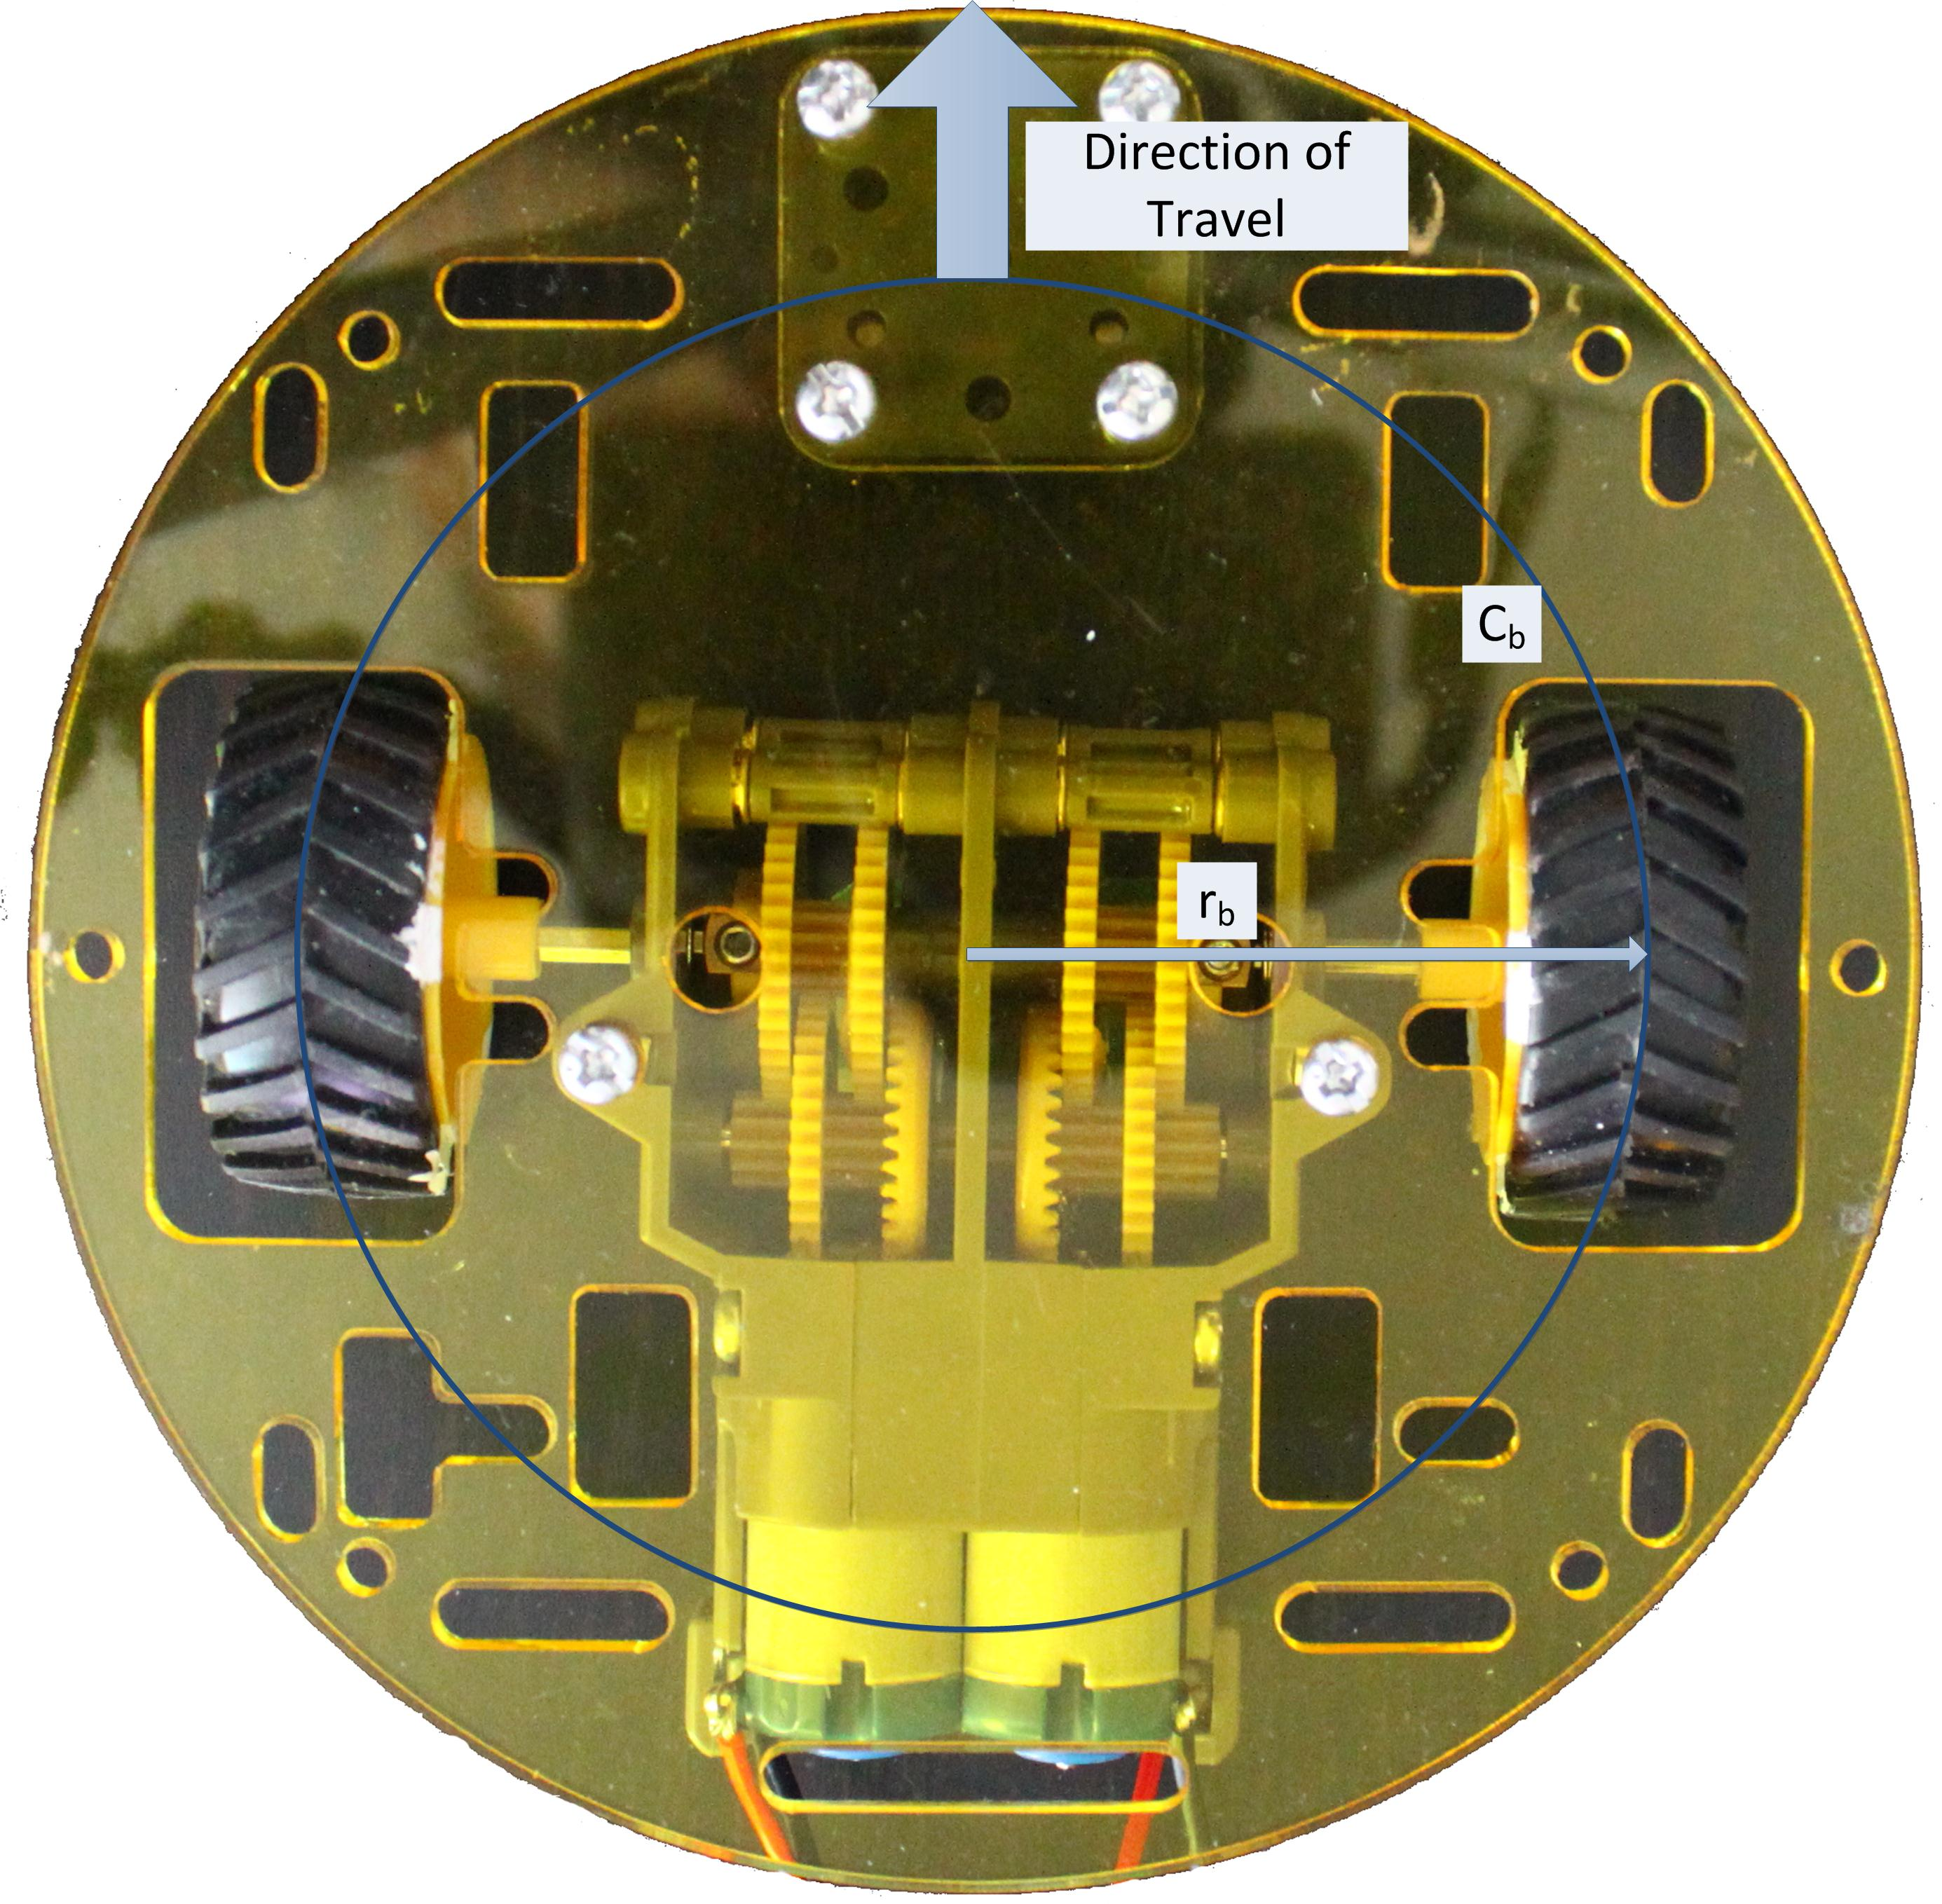
\includegraphics[width = \textwidth, keepaspectratio]{./Figures/Robotbase_top_annot.jpg} }
\subfigure[Side View of robot base showing dimensions of interest\label{fg:RobotBase:Side}]{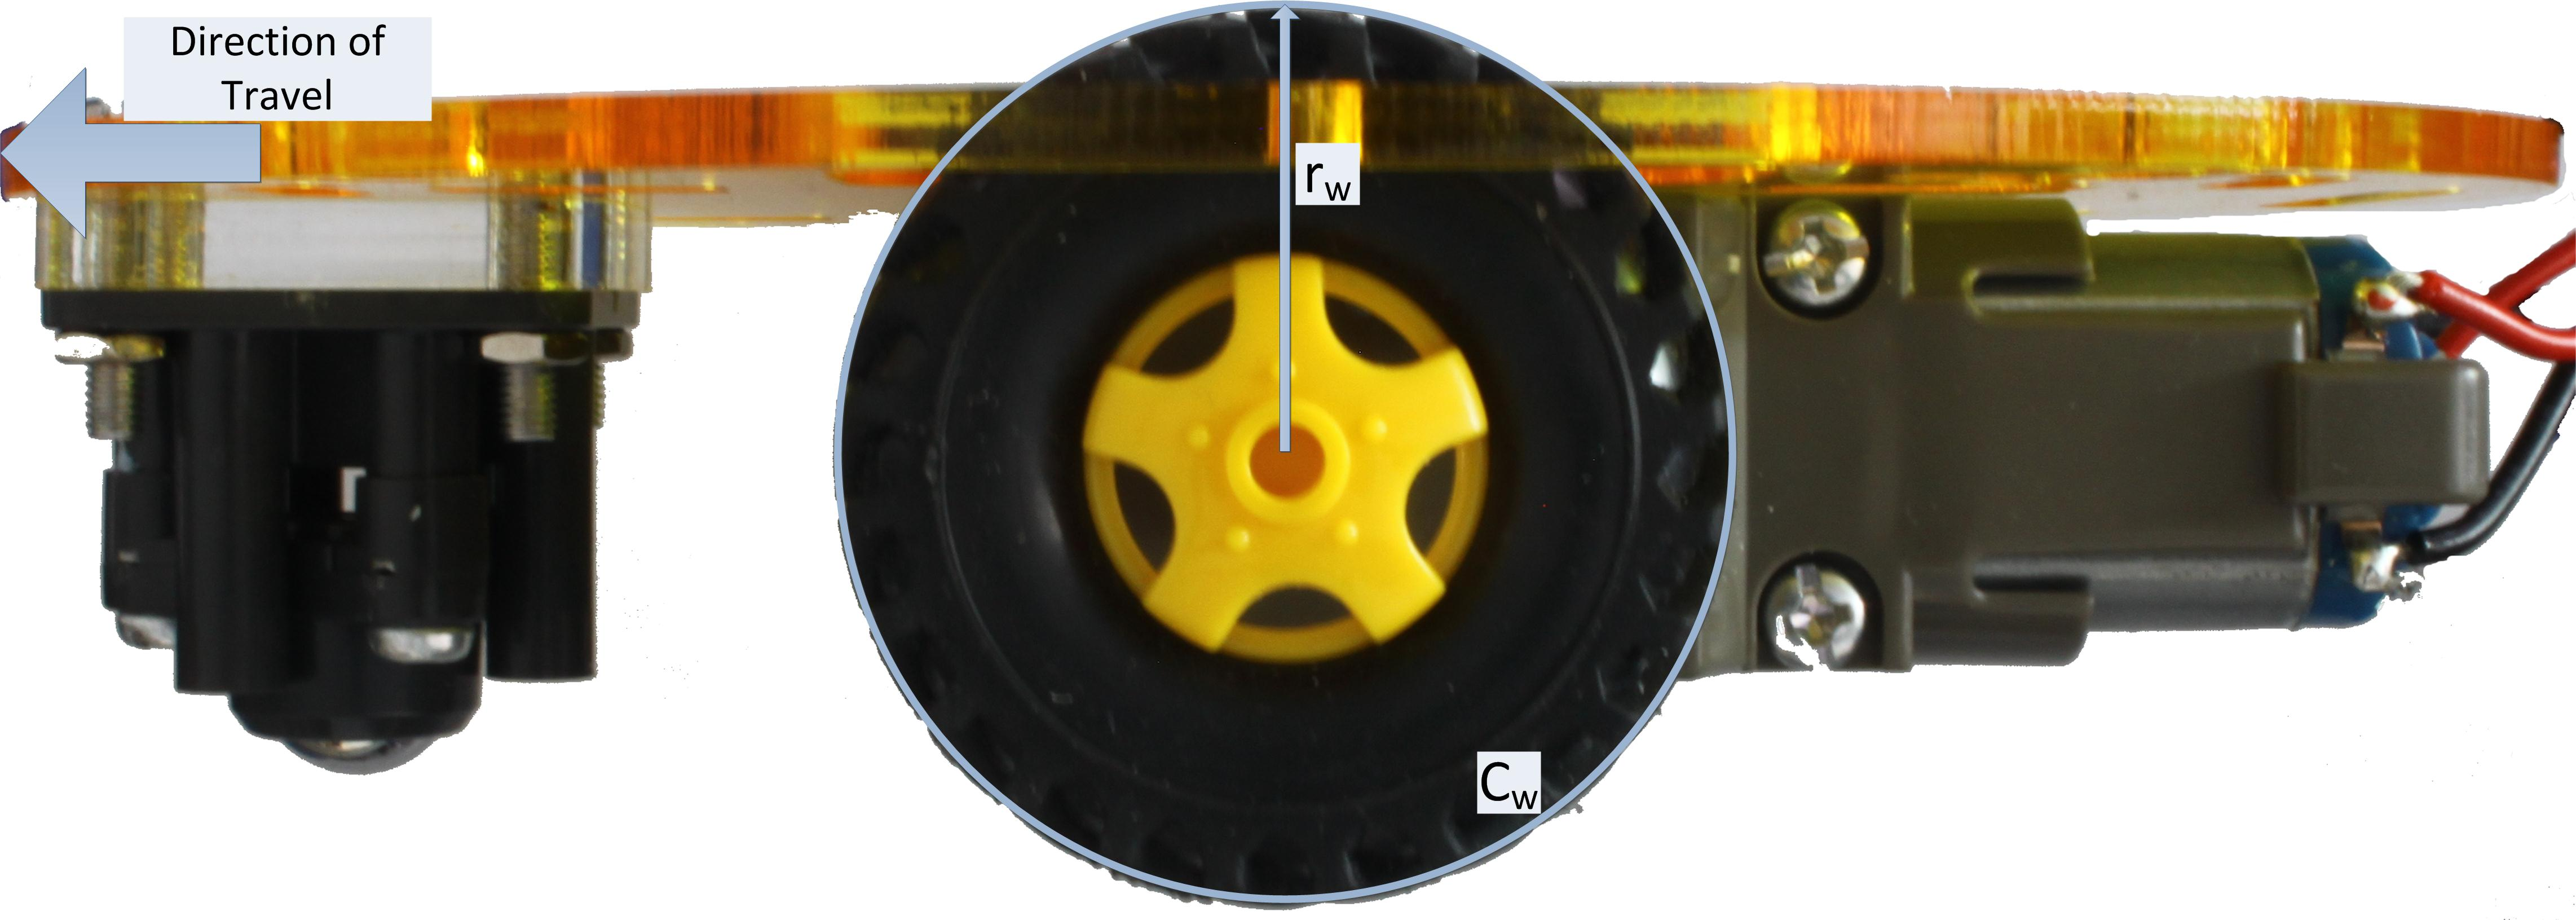
\includegraphics[width = \textwidth, keepaspectratio]{./Figures/Robotbase_side_annot.jpg} }
\caption{Dimensions of Interest for Robot Movement}
\label{fig:RobotBase_Annotated}
\end{figure}

 

The final code can be seen in appendix \ref{Chapter:AppendixC:Code}. \textit{Motor\_Init} method must be called before operation can occur. This sets up the PWM and analogue comparators. Methods \textit{Motors\_Move} and \textit{Motors\_Rotate} are the methods that can be called to move in a straight line or rotate on the spot. They both take an input which is a signed integer of either the distance to move (in millimetres) or the angle to rotate (in degrees, positive is a clockwise movement). They both return the actual movement distances, due to the low resolution of the system.


\subsection{Testing}\label{Section:MotorTest}
%\inote{Test Rotation}

To test the motor system, different distances were given to the movement method. The method prints how many counts will be moved. The actual distance moved was then measured and repeated four times. Table \ref{table:results:motor:distance} and figure \ref{fig:results:motor:distance} show the results of this test. The results show that the maximum error observed is $4.52\%$, which related to $4.5mm$. This error is acceptable as a half centimetre error over 10cm will not impact the performance of the robot. The error is calculated from the actual distance predicted to move. 


\begin{table}
\caption{Results of Motor Distance Test}
\label{table:results:motor:distance}
\begin{tabular}{|p{2.5cm}|p{2.5cm}|p{2.5cm}|p{2.5cm}|p{2.5cm}|} \hline
Distance Specified (mm) &	Number of Counts Calculated	& 	Counts $\times$ Resolution (mm)	& 	Average Measured Distance Moved (mm)	&	Error (\%) \\ \hline
50						&	4							&	46.4							&	47.25									&	1.83		\\
75						&	6							&	69.6							&	70.75									&	1.65		\\
100						&	8							&	92.8							&	97.0									&	4.52		\\
120						&	10							&	116.0							&	113.25									&	2.37		\\
150						&	12							&	139.2							&	141.0									&	1.29		\\
170						&	14							&	162.4							&	161.5									&	0.55		\\
200						&	17							&	197.2							&	201.5									&	2.18		\\
250						&	21							&	243.6							&	244.5									&	0.37		\\
300						&	25							&	290.0							&	290.75									&	0.26		\\ \hline
\end{tabular}
\end{table}

\begin{figure}
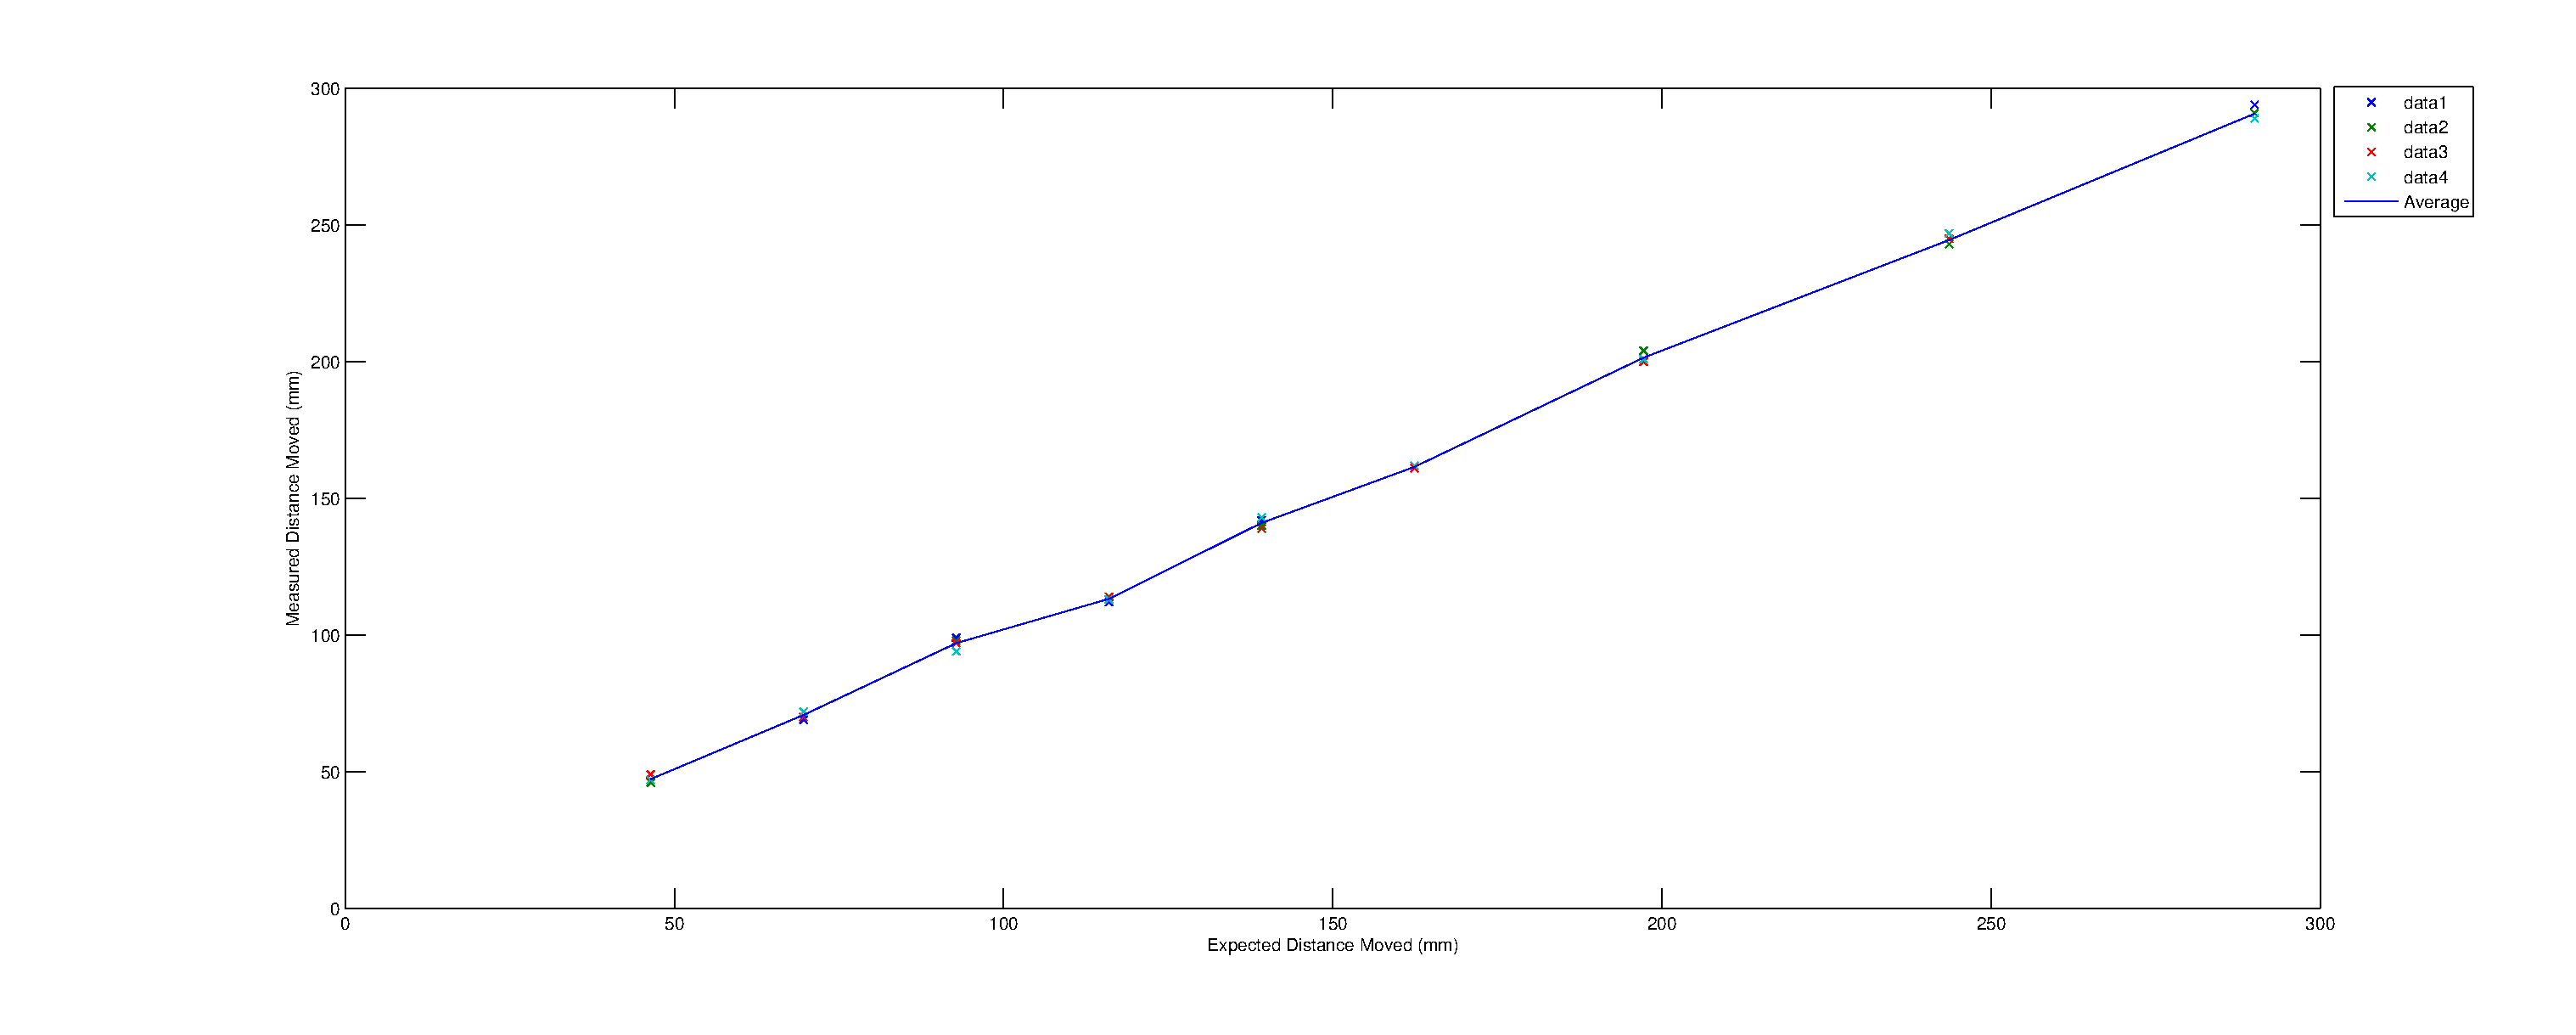
\includegraphics[width=\textwidth]{Figures/Motor_Distance.eps}
\caption{A plot of Expected Distance against the measured data. Line indicates the average of the data at each point.}
\label{fig:results:motor:distance}
\end{figure}

A problem was seen that the robot moved in a slight arc. Speed tests were done on the wheel by measuring the total time taken to complete eight full revolutions, the equivalent of moving 928mm. The results and the calculated wheel speeds can be seen in table \ref{table:results:motor:speed}. It shows that the left motor runs slightly faster than the right, even though the PWM duty cycle is the same. A controller could be implemented to correct this error during operation. However, over the distances covered, the error introduced by this is small enough to neglect. 

\begin{table}
\caption{Results of motor speed test}
\label{table:results:motor:speed}
\centering
\begin{tabular}{|c|c|c|} \hline
Wheel &	Total Time Elapsed ($s$) & Calculated Speed ($mm.s^{-1}$) \\ \hline
Left & 44.6		&	20.8 \\ \hline
Right & 49.6	&	18.7 \\ \hline
\end{tabular}
\end{table}

\subsection{Conclusion}
Due to the low resolution of the sensor (10 counts per revolution), there is a minimum distance that can be moved and a minimum angle of rotation, shown in equations \eqref{eq:Resolution:Distance} and \eqref{eq:Resolution:Angle} respectively. These show a that greater distance resolution could be obtained by decreasing the wheel size or increasing $\gamma$ and a greater rotational resolution could be obtained by the same as distance, or by increasing the distance the wheels are from the centre of the robot. In general, the ratio $C_w:\gamma$ should be as large as possible to obtain the best resolution for movement.


\begin{equation}\label{eq:Resolution:Distance}
\Delta_{\delta} = \frac{C_w}{\gamma} = 12mm
\end{equation}
\begin{equation}\label{eq:Resolution:Angle}
\Delta_{\theta} = \frac{360 \times C_w}{\gamma \times C_b} \approx 15^\circ 
\end{equation}

This method lacks on two points - lack of speed control and accuracy.
A better controller could be implemented to help move at different speeds. This could use the remaining number of counts to gradually slow the speed of the motors down as well as correct the speed mismatch between the wheels. A PID controller could be implemented if greater accuracy is needed quicker, at the expense of computation time and potential overshoot. 

Rotary encoders could be used to detect the direction of wheels as well. A good, but more costly, alternative would be the HUB-ee wheel by \cite{Creative_Robotics}, which includes a 120 point quadrature encoder and sensor, motor driver and a geared motor all within the wheel. These wheels have 12 times the accuracy as the method described here and a similar interface. 
 
Given that the robot does not need to move any more accurately that to 1cm, this method has proved to be cheap and successful. The robot is able to move a distance with reasonable accuracy, but to a fairly low resolution.

\section{PCB Development}\label{Section:PCB_Dev}
\subsection{Circuit Design}

Figure \ref{fig:Hierarchical} shows a basic hierarchy of the robot. Each pin on the UC3C can have one of up to six special functions, as well as being a GPIO pin.  Table \ref{table:UC3C:Pinout} shows the pinout for the microcontroller used. 
\begin{figure}
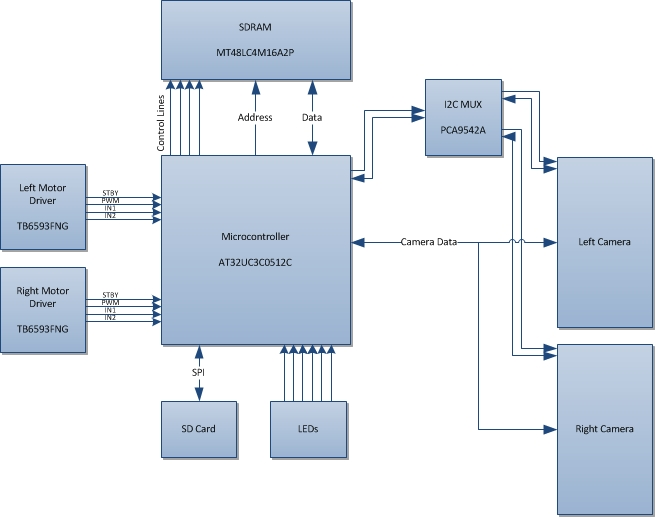
\includegraphics[width=\textwidth]{Figures/hierarchy.jpg}
\caption{A hierarchical diagram of the robot}
\label{fig:Hierarchical}
\end{figure}

\begin{table}
\centering
\caption{The Pinout of the AVR for the circuit. `-' means unavailable and blank means unused}
\label{table:UC3C:Pinout}
%\begin{tabular}{|p{1.2cm}|p{3cm}|p{3cm}|p{3cm}|p{3cm}|}\cline{2-5}
\begin{tabular}{|c|c|c|c|c|}\cline{2-5}
\multicolumn{1}{c|}{ } & \multicolumn{4}{|c|}{Port} \\ \hline
Pin & A & B & C & D \\ \hline
0&TCK&CAMERA\_ 0&&EBI-DATA13\\
1&TDI&CAMERA\_ 1&&EBI-DATA14\\
2&TDO&CAMERA\_2&SDA&EBI-DATA15\\
3&TMS&CAMERA\_3&SCL&EBI-ADDR0\\
4&USB ID&CAMERA\_4&USART TXD&EBI-ADDR1\\
5&&CAMERA\_5&USART RXD&EBI-ADDR2\\
6&AC R&CAMERA\_6&&EBI-ADDR3\\
7&AC R&CAMERA\_7&EBI NCS3&EBI-ADDR4\\
8&AC L&STBY1&EBI NCS0&EBI-ADDR5\\
9&AC L&IN11&EBI-ADDR23&EBI-ADDR6\\
10&VSYNC0&IN12&EBI-ADDR22&EBI-ADDR7\\
11&ADCREF&PWM1&EBI-ADDR21&EBI-ADDR8\\
12&&&EBI-ADDR20&EBI-ADDR9\\
13&&PWM2&&EBI-SDCK\\
14&&IN22&EBI-SDCKE&EBI-ADDR10\\
15&RRST0&IN21&EBI-SDWE&EBI-ADDR11\\
16&ADCREF&STBY2&EBI-CAS&EBI-ADDR12\\
17&-&&EBI-RAS&EBI-ADDR13\\
18&-&&EBI-SDA10&EBI-ADDR14\\
19&RCLK0&SPI-MOSI&EBI-DATA0&EBI-ADDR15\\
20&WEN0&SPI-MISO&EBI-DATA1&EBI-ADDR16\\
21&WRST0&SPI-SCK&EBI-DATA2&EBI-ADDR17\\
22&RRST1&SPI-CS3&EBI-DATA3&EBI-ADDR18\\
23&RCLK1&SPI-CS2&EBI-DATA4&EBI-ADDR19\\
24&WEN1&SPI-CS1&EBI-DATA5&EBI-NWE1\\
25&WRST1&SPI-CS0&EBI-DATA6&EBI-NWE0\\
26&VSYNC1&SD- DETECT&EBI-DATA7&EBI-NRD\\
27&NOE1&&EBI-DATA8&EBI NCS1\\
28&NOE0&&EBI-DATA9&EBI NCS2\\
29&&&EBI-DATA10&\\
30&-&CLK&EBI-DATA11&EBI-NWAIT\\
31&-&CLK&EBI-DATA12&-\\ \hline

\end{tabular}
\end{table}

The circuit diagram for Revision A can be seen in section \ref{sch:Columbus:CircuitDiagram}. The schematic for the SDRAM and values and locations of decoupling capacitors were used from the schematic of the UC3C-EK development board \citep{Atmel:UC3CEK}. 
\subsection{PCB Design}
The PCB was designed using EAGLE CAD Software. A four layer board was decided to be used to reduce the number of tracks and more easily supply power and ground to the devices. Layer two is a $3.3V$ plane and layer three is a ground plane. A ground plane is also on the top and bottom layers to help eliminate any ground bounce that could occur. 

The SDRAM uses the EBI protocol. In high speed systems, care is often taken to equalise track lengths \citep{liu2004equalization}. The UC3C maximum clock frequency is 33MHz (with no wait states), which is not fast enough to cause any track equalisation problems. Care, however, was taken on the USB lines to ensure correct impedance and the tracks lengths matched to each other.

Tracks were routed in order of priority, starting with the UC3C, SDRAM and cameras. All other devices were then routed (\itc multiplexer, SD card, motor drivers etc). As a precaution, spare pins from the UC3C were routed to headers (J8 and J9, so that additions could be done if a pinout or connection was found to be incorrect. UART, \itc and SPI connections were routed to headers J7, J4 and J5 respectively so logic analysers and a COM Port could be attached easily for debugging, or so that extra devices could be added onto the respective protocols for future developments. 

Passives used were all surface mount of either 0603 or 1206 size to save space on the board. All headers used were 0.1'' spaced for easy connections and a mini B USB socket was added to power the robot, program via the bootloader or so that the robot could potentially act as a USB device. 

The layout of components was important. The cameras needed to be as far apart as possible and at the front of the PCB. The motor drivers were situated toward the back of the PCB and headers were added to connect the motors to. The optosensors were positioned such that they could be mounted directly on the PCB and be in the correct position to sense the wheels. Mounting holes were also added onto the board so the PCB could be mounted on to the robot base easily. The overall dimensions of the PCB were $100mm \times 70mm$. A full list of components and cost of each is documented in Appendix \ref{Appendix:Costings}


Finally, the name \textit{``The Columbus''} was decided on as the original application for the project was a mapping robot that would search out an unknown area, so the robot was named after Christopher Columbus who explored and navigated parts of the American continents which were unknown at the time. The Eagle CAD Diagram of the PCB can be seen in Appendix \ref{Appendix:PCB}. The PCB was manufactured by \cite{PCBCart}. The PCB cost \pounds 205 to manufacture and ship. A photo of the PCB can be seen in figure \ref{fig:PCB:Bare}. 

\begin{figure}
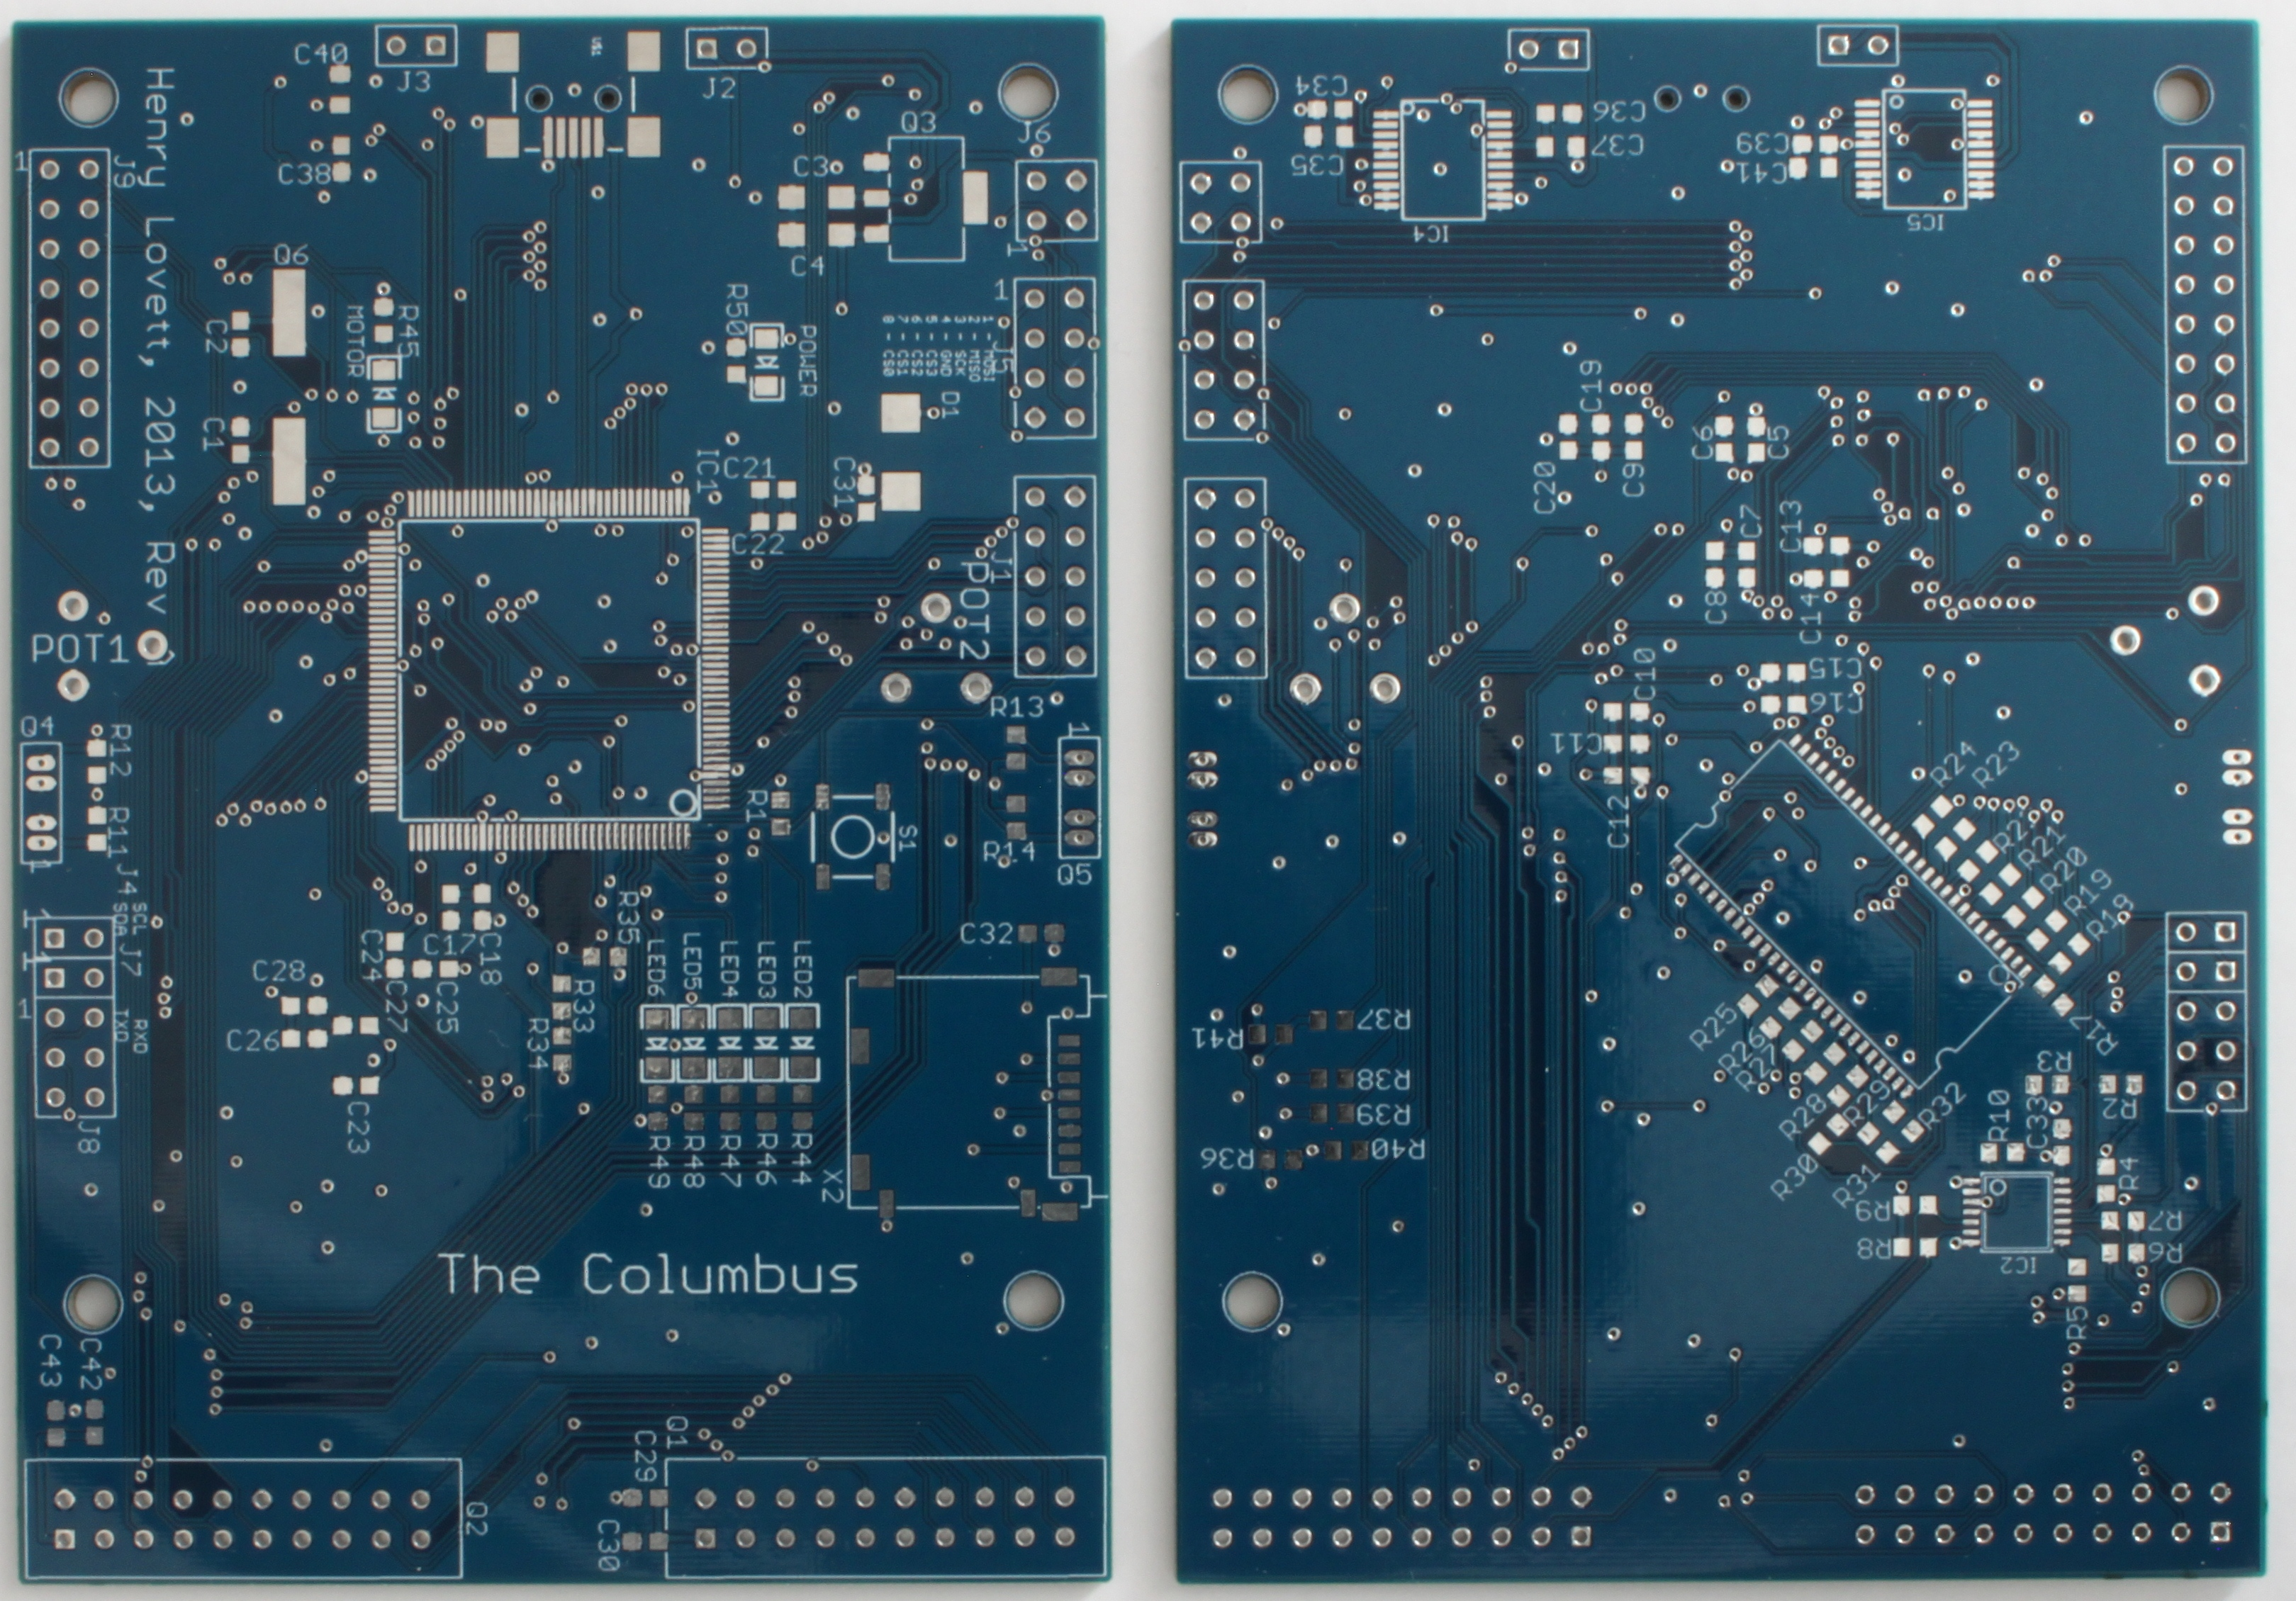
\includegraphics[width=\textwidth]{./Figures/PCB_Bare.jpg}
\caption{PCB with no components. Left: Top View. Right: Bottom View}
\label{fig:PCB:Bare}
\end{figure}

\inote{Considerations - Power consumption of devices not exceeding VReg}

\subsection{PCB Testing}
A program was written to test all the devices on the PCB. The following tests are done and are explained in the subsequent sections:
\begin{enumerate}
\item[\ref{UART:Test}] UART Send and Receive
\item[\ref{SD:Test}] SD Card 
\item[\ref{LED:Test}] LEDs 
\item[\ref{SDRAM:Test}] SDRAM 
\item[\ref{I2C:Test}] \itc 
\item[\ref{Camera:Test}] Camera 
\item[\ref{Motor:Test}] Motor 
\end{enumerate}


\subsubsection{UART Test}\label{UART:Test}
When the test program begins, the microcontroller waits for a character input. All characters are echoed back. This enables the user to check the communications work. Once a carriage return key is received ($D_{16}$), the test program continues. Listing \ref{lst:UARTTestCode} shows the test code for the UART protocol.

\lstinputlisting[style=C,caption=UART Test Code,label={lst:UARTTestCode},frame=single,numbers=left,tabsize=2,breaklines=true, firstline=110,lastline=121]{../Code/ColumbusTest/ColumbusTest/src/main.c}


\subsubsection{SD Card Test}\label{SD:Test}
The Atmel Software Framework \citep{Atmel:ASF} provided drivers and code for SPI communications and use of a FAT32 file system. The code was configured to use the correct chip select pin for the SD Card and the correct SPI Bus. The test consisted of initialising the memory, reading the capacity of the card and printing it to the user. 

The AVR then proceeds to delete any previous log file, create a new log file and writes \textit{``Columbus Tester''} to it. The first 8 characters, which should be \textit{``Columbus''} are read back and checked.
\lstinputlisting[style=C,caption=UART Test Code,label={lst:SDTestCode},frame=single,numbers=left,tabsize=2,breaklines=true, firstline=124,lastline=196]{../Code/ColumbusTest/ColumbusTest/src/main.c}

This exercises all basic file I/O functions, creating, reading and writing and checks that they work.

\subsubsection{LED Test}\label{LED:Test}
All LEDs are turned on for 1 second, and then turned off. The user should check this occurs. It verifies that all the LEDs are functional and correctly mounted. The Power LED should be on when power is supplied to the PCB. 

\subsubsection{SDRAM Test}\label{SDRAM:Test}
The SDRAM test consists of initialising the SDRAM, calculating the SDRAM size, writing a unique test pattern to the whole memory, and then reading it back and checking it. The total number of errors are reported. 

The test was adapted from an example application from the ASF \citep{Atmel:ASF}. The code can be seen in listing \ref{lst:SDRAMTestCode}. It consists of two \textit{for} loops. In the first, the iteration number is assigned to the memory location. The second loop reads back the data and checks it is correct. An int, \textit{noErrors}, is used to count errors. 

\lstinputlisting[style=C,caption=SDRAM Test Code,label={lst:SDRAMTestCode},frame=single,numbers=left,tabsize=2,breaklines=true, firstline=217,lastline=258]{../Code/ColumbusTest/ColumbusTest/src/main.c}

\subsubsection{\itc Test}\label{I2C:Test}
The \itc test checks the bus for devices. It prints out a table showing the address of any devices that acknowledges a probe. A probe is a set up to write to the address. If a device exists on the line, it should acknowledge \citep{Philips:I2C}. The test is done three times, with no channel selected on the \itc multiplexer, with channel 0 selected and with channel 1 selected. The two addresses expected at $21_{16}$ for the OV7670 Camera and $74_{16}$ for the \itc multiplexer. The camera should only acknowledge when the \itc multiplexer has the relevant channel selected. Listing \ref{lst:TWITestCode} shows the test code for the \itc bus and listing \ref{lst:I2CTest} shows the result from the full bus scan with channel 0 selected. The cameras are both checked to exist.
\lstinputlisting[style=C,caption=\itc Test Code,label={lst:TWITestCode},frame=single,numbers=left,tabsize=2,breaklines=true, firstline=268,lastline=315]{../Code/ColumbusTest/ColumbusTest/src/main.c}

\begin{lstlisting}[caption={Result of \itc bus scan with Channel 0 of the \itc multiplexer selected},label={lst:I2CTest}]
Scanning Channel 0
h 0 1 2 3 4 5 6 7 8 9 A B C D E F
0 - - - - - - - - - - - - - - - -
1 - - - - - - - - - - - - - - - -
2 - A - - - - - - - - - - - - - -
3 - - - - - - - - - - - - - - - -
4 - - - - - - - - - - - - - - - -
5 - - - - - - - - - - - - - - - -
6 - - - - - - - - - - - - - - - -
7 - - - - A - - - - - - - - - - -
\end{lstlisting}

\subsubsection{Camera Test}\label{Camera:Test}

This test consists of initialising both cameras and checking it succeeds. Two photos are then taken and stored to the SD card. Success or failure of the methods is sent to the debug terminal. Two images should exist on the SD card from the two cameras. Listing \ref{lst:CameraTestCode} shows the code to conduct this test.
\lstinputlisting[style=C,caption=Camera Test Code,label={lst:CameraTestCode},frame=single,numbers=left,tabsize=2,breaklines=true, firstline=316,lastline=338]{../Code/ColumbusTest/ColumbusTest/src/main.c}

\subsubsection{Motor Driver Test}\label{Motor:Test}
An extensive test of the motor driver is discussed in section \ref{Section:MotorTest}. The test code in this application resets the motors so that they are aligned to a white tab on the wheel. This code can be seen in listing \ref{lst:MotorTestCode}. The robot should move no further than 1cm to reach a white tab and the motors should drive forward. This test is useful here to ensure the motors are connected the correct way around and that the potentiometers are set to an appropriate level.

\lstinputlisting[style=C,caption=Motor Test Code,label={lst:MotorTestCode},frame=single,numbers=left,tabsize=2,breaklines=true, firstline=339,lastline=346]{../Code/ColumbusTest/ColumbusTest/src/main.c}

\subsection{PCB Faults}
During the build and test of the PCB, a number of faults were found. Each is explained and the solution for the problem given. 
\subsubsection{TCRT1010 Footprint}
The holes in the footprint for the optosensor were not large enough. This was a minor problem as the sensor was soldered in a surface mount style. This didn't affect the location of the sensor so had no other implications other than the connection being weaker than it should be. 
\subsubsection{SDRAM Footprint}
The SDRAM footprint made was done exactly to the specification of the pad size and locations with no consideration for soldering. This meant the chip fits exactly on to the footprint and made soldering difficult as pads had to be preloaded with solder and the device's pins were heated and bound to the solder. It also put the device at risk as more heat had to be used that usually necessary. Figure \ref{fig:SDRAM_Err} shows the SDRAM chip slightly offset against the footprint. It can be seen that there is no extra space on the pad to be able to easily solder the device. Though this made building difficult and increased soldering errors, it had no impact on the operation of the device.

\begin{figure}
\centering
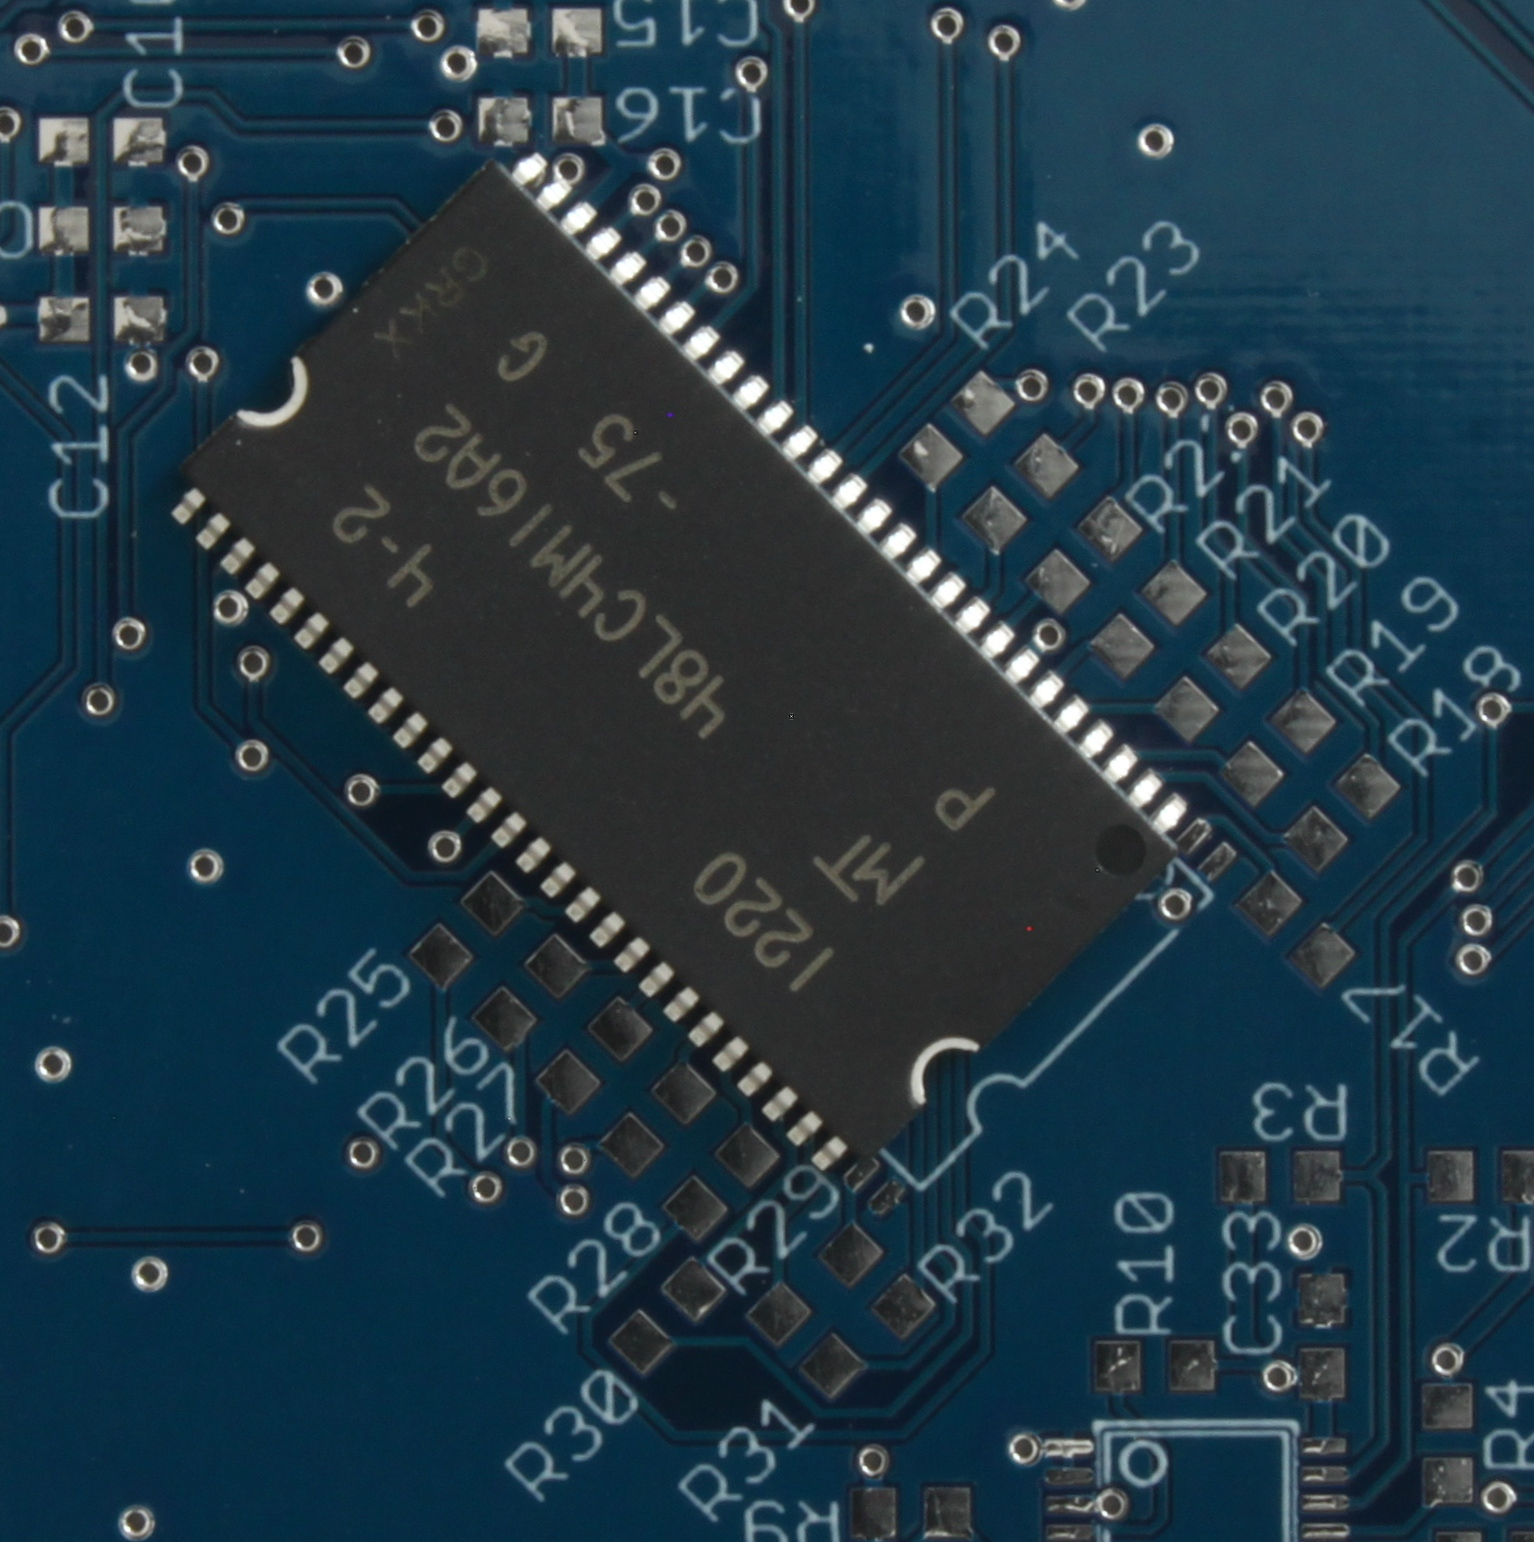
\includegraphics[width=\textwidth / 2]{./Figures/PCB_SDRAM.jpg}
\caption{SDRAM Chip shown against its footprint.}
\label{fig:SDRAM_Err}
\end{figure}

To avoid this, existing footprints could be used from other libraries, or double checking the footprints made. The problem meant extra care during soldering had to be taken but has not impeded the operation of the device. 

\subsubsection{SDRAM Chip Select}
The code was prototyped on the Atmel UC3C-EK development board prior to the PCB arriving. This used chip select 1 for the SDRAM and the PCB was designed using chip select 0. When the PCB was built, the code did not work. To diagnose this problem, the control lines of the SDRAM were probed with a logic analyser. On the UC3C-EK, the bus was busy with refresh cycles outside of SDRAM access. On the Columbus, no activity was seen. 

The reason the correct control wasn't being seen was due to the UC3C device having a dedicated SDRAM controller, attached only to chip select line 1. Chip select 1 was available on an external pin, and the via on the CS0 and CS1 lines were close to each other. Therefore, to overcome the problem, a small enamelled wire was soldered to join the two vias together. This solved the problem and the correct signals were then seen on the control lines. The patch can be seen in figure \ref{fig:PCB:Bottom}. 

This fault was caused by not reading the datasheet carefully and ignoring a proven circuit diagram. Operation of the device was not hindered and the fix was simple.

\subsubsection{SDRAM Data Line Resistors}
Once the chip select problem was solved, data returned was unreliable. The SDRAM is word (32 bit) addressed, but accessed in 16 bits. Each SDRAM access, therefore, consisted of two access cycles. 
Upon investigation of this problem, the 14th, 15th, 30th and 31st (top two bits of each 16 bit access) seemed to read as a 1 the majority of the time. This result wasn't repeatable and sometimes returned correct data. The other bits of the data were always correct. Table \ref{table:SDRAM_Err} shows some examples of the problematic data bits. The data written should match the data read back. 

\begin{table}[!ht]
\caption{A table showing examples of the incorrect data returned from the SDRAM}
\label{table:SDRAM_Err}
\begin{tabular}{|c|c|}\hline
Data Written							&	Data Read \\\hline
00000000 00000000 00000000 00000000		&	\textcolor{red}{11}000000 00000000 \textcolor{red}{11}000000 00000000 \\
00001111 00001111 00001111 00001111		&	\textcolor{red}{11}001111 00001111 \textcolor{red}{11}001111 00001111 \\\hline
\end{tabular}
\end{table}

The problem was traced to resistors \textbf{R31} and \textbf{R32}. They were soldered on incorrectly so that the two data lines of the SDRAM were connected together and the two AVR GPIO pins were connected together. Data was then read back from, effectively, a high impedance line and therefore varied. Once the resistors were soldered correctly, the issue no longer persisted and the whole SDRAM test passed. By utilising the soldermask more, device orientations could be added to ensure correct placement. This can be extended to other devices, such as diodes and capacitors, especially in densely populated areas of the PCB. 

\subsubsection{Camera Interrupt Line}

As discussed in section \ref{Section:Camera}, the OV7670 needs an interrupt line to synchronise quickly to the start of the frame and is done by using an interrupt line. The UC3C has 9 external interrupt lines. On the PCB, interrupt lines 0 and 1 were used for this control.

Interrupt line 1 was easily configured and worked as expected. However, interrupt 0 did not seem to trigger the interrupt service routine. It was found that interrupt 0 was a ``Non Maskable Interrupt'' which has specific uses and cannot be used in to trigger a method. 

The external interrupt 4 pin was wired to Junction 8 on the PCB. A wire was attached to the camera's VSYNC line and attached to the relevant pin on the header. The operation was then easily obtained and the VSYNC line triggered correctly.

This issues would have been avoided with more understanding of the device before hand and checking the datasheet. The patch can also be seen in figure \ref{fig:PCB:Bottom}.


\subsubsection{Motor Driver Footprint}

An error was made in creating the device for the TB6593FNG Motor Driver in EAGLE. The chip has two outputs and each motor output has two pins to drive each pin of the motor. The pin assignment was mixed up when created and connected the two outputs together. Figure \ref{fig:Motor:Error} shows the track errors on one of the motor drivers. 

\begin{figure}
\centering
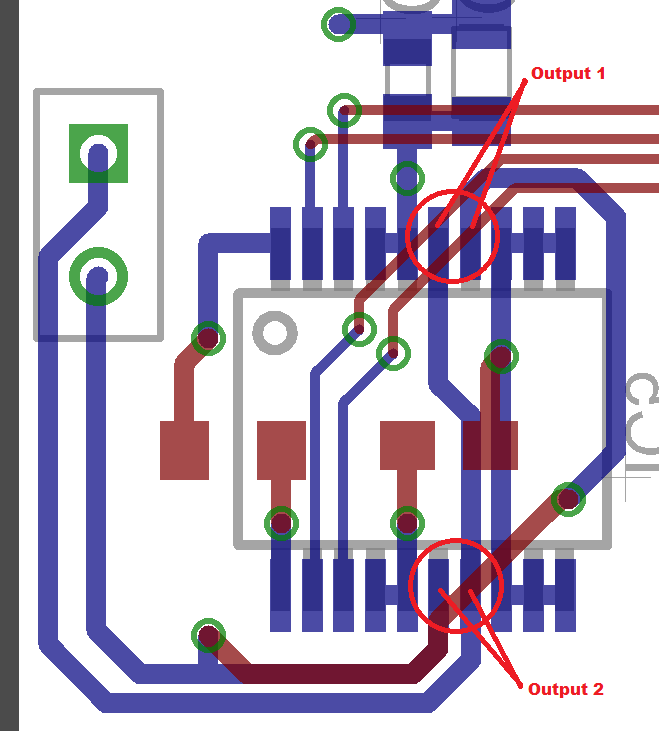
\includegraphics[width = \textwidth /2]{./Figures/MotorDriver_error.png}
\caption{Motor Driver error. Outputs incorrectly connected}
\label{fig:Motor:Error}
\end{figure}

To solve this, pins 7 and 14 were lifted and removed so that output 1 and output 2 were not connected together. The devices were not damaged in the process of testing this and the motors functioned correctly after the modification. Double checking the footprints made against the datasheet would have avoided this problem. No impact to the operation of the drivers has been seen, but the patch may hinder the devices ability to sink current to the motors when driving at higher speeds. 

\subsection{PCB Conclusions}
A number of faults were made in the PCB design. They are:
\begin{itemize}
\item TCRT1010 footprint
\item SDRAM footprint
\item SDRAM chip select line
\item SDRAM data line resistors
\item Camera interrupt line
\item Motor driver footprint
\end{itemize}
Three of the faults were due to footprint errors. Consulting the data sheets or using existing footprints would have avoided these problems. Two circuit errors were due to special operations of pins on the UC3C. More experience with this device could have prevented this but the errors were easily patches. By utilising the soldermask more would prevent errors during building. 

For future PCBs, more care will be taken in circuit design, with prototyping of circuits with the hardware that will be used. This will highlight any pin specific operations (e.g. the non maskable interrupt) and reduce debugging post production. The effectiveness of a soldermask is also apparent, so more time spent on utilising this would be helpful during assembly.

The PCB itself, was a success. It was a complex PCB with many potential things that could have gone wrong. All devices are functional (with a few small modifications) on the PCB so firmware development could continue with all hardware able to be used. Figure \ref{fig:PCB:Built} shows the fully assembled PCB with the modifications needed.

\begin{figure}
\centering
\subfigure[Top view of built PCB\label{fig:PCB:Top}]{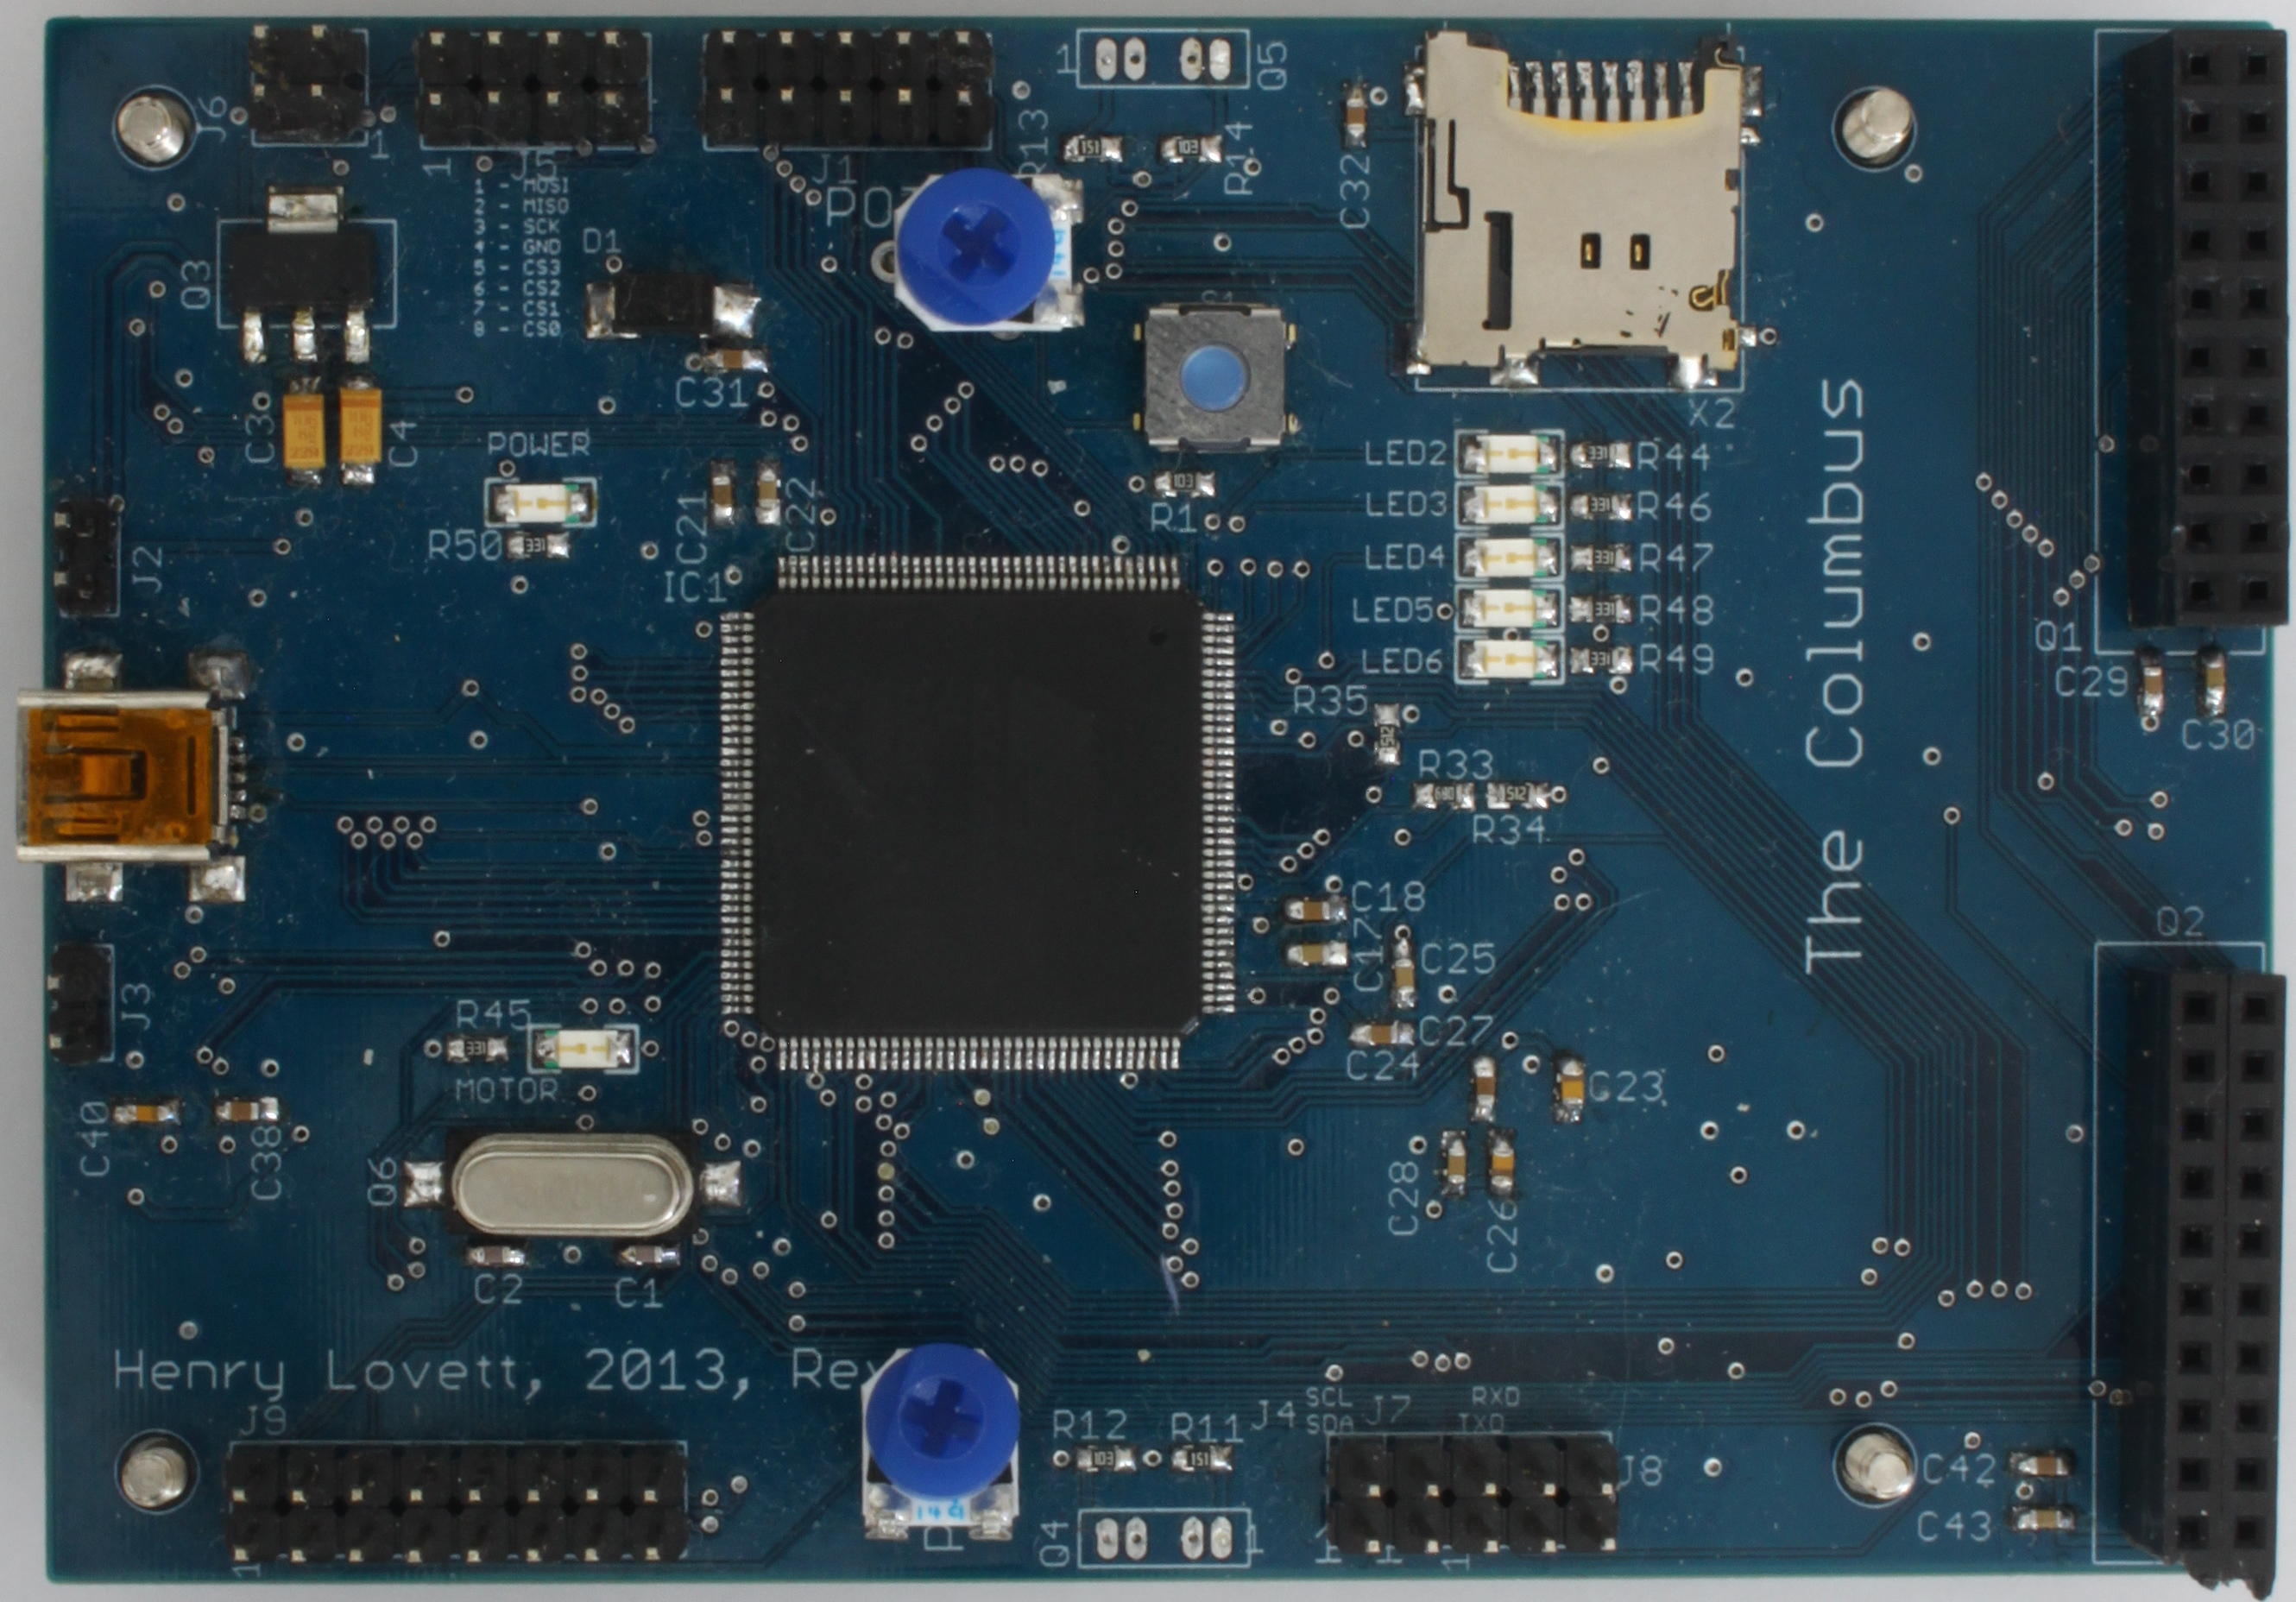
\includegraphics[width = \textwidth, keepaspectratio]{./Figures/PCB_Top.jpg} }
\subfigure[Bottom view of built PCB with SDRAM chip select patch \label{fig:PCB:Bottom}]{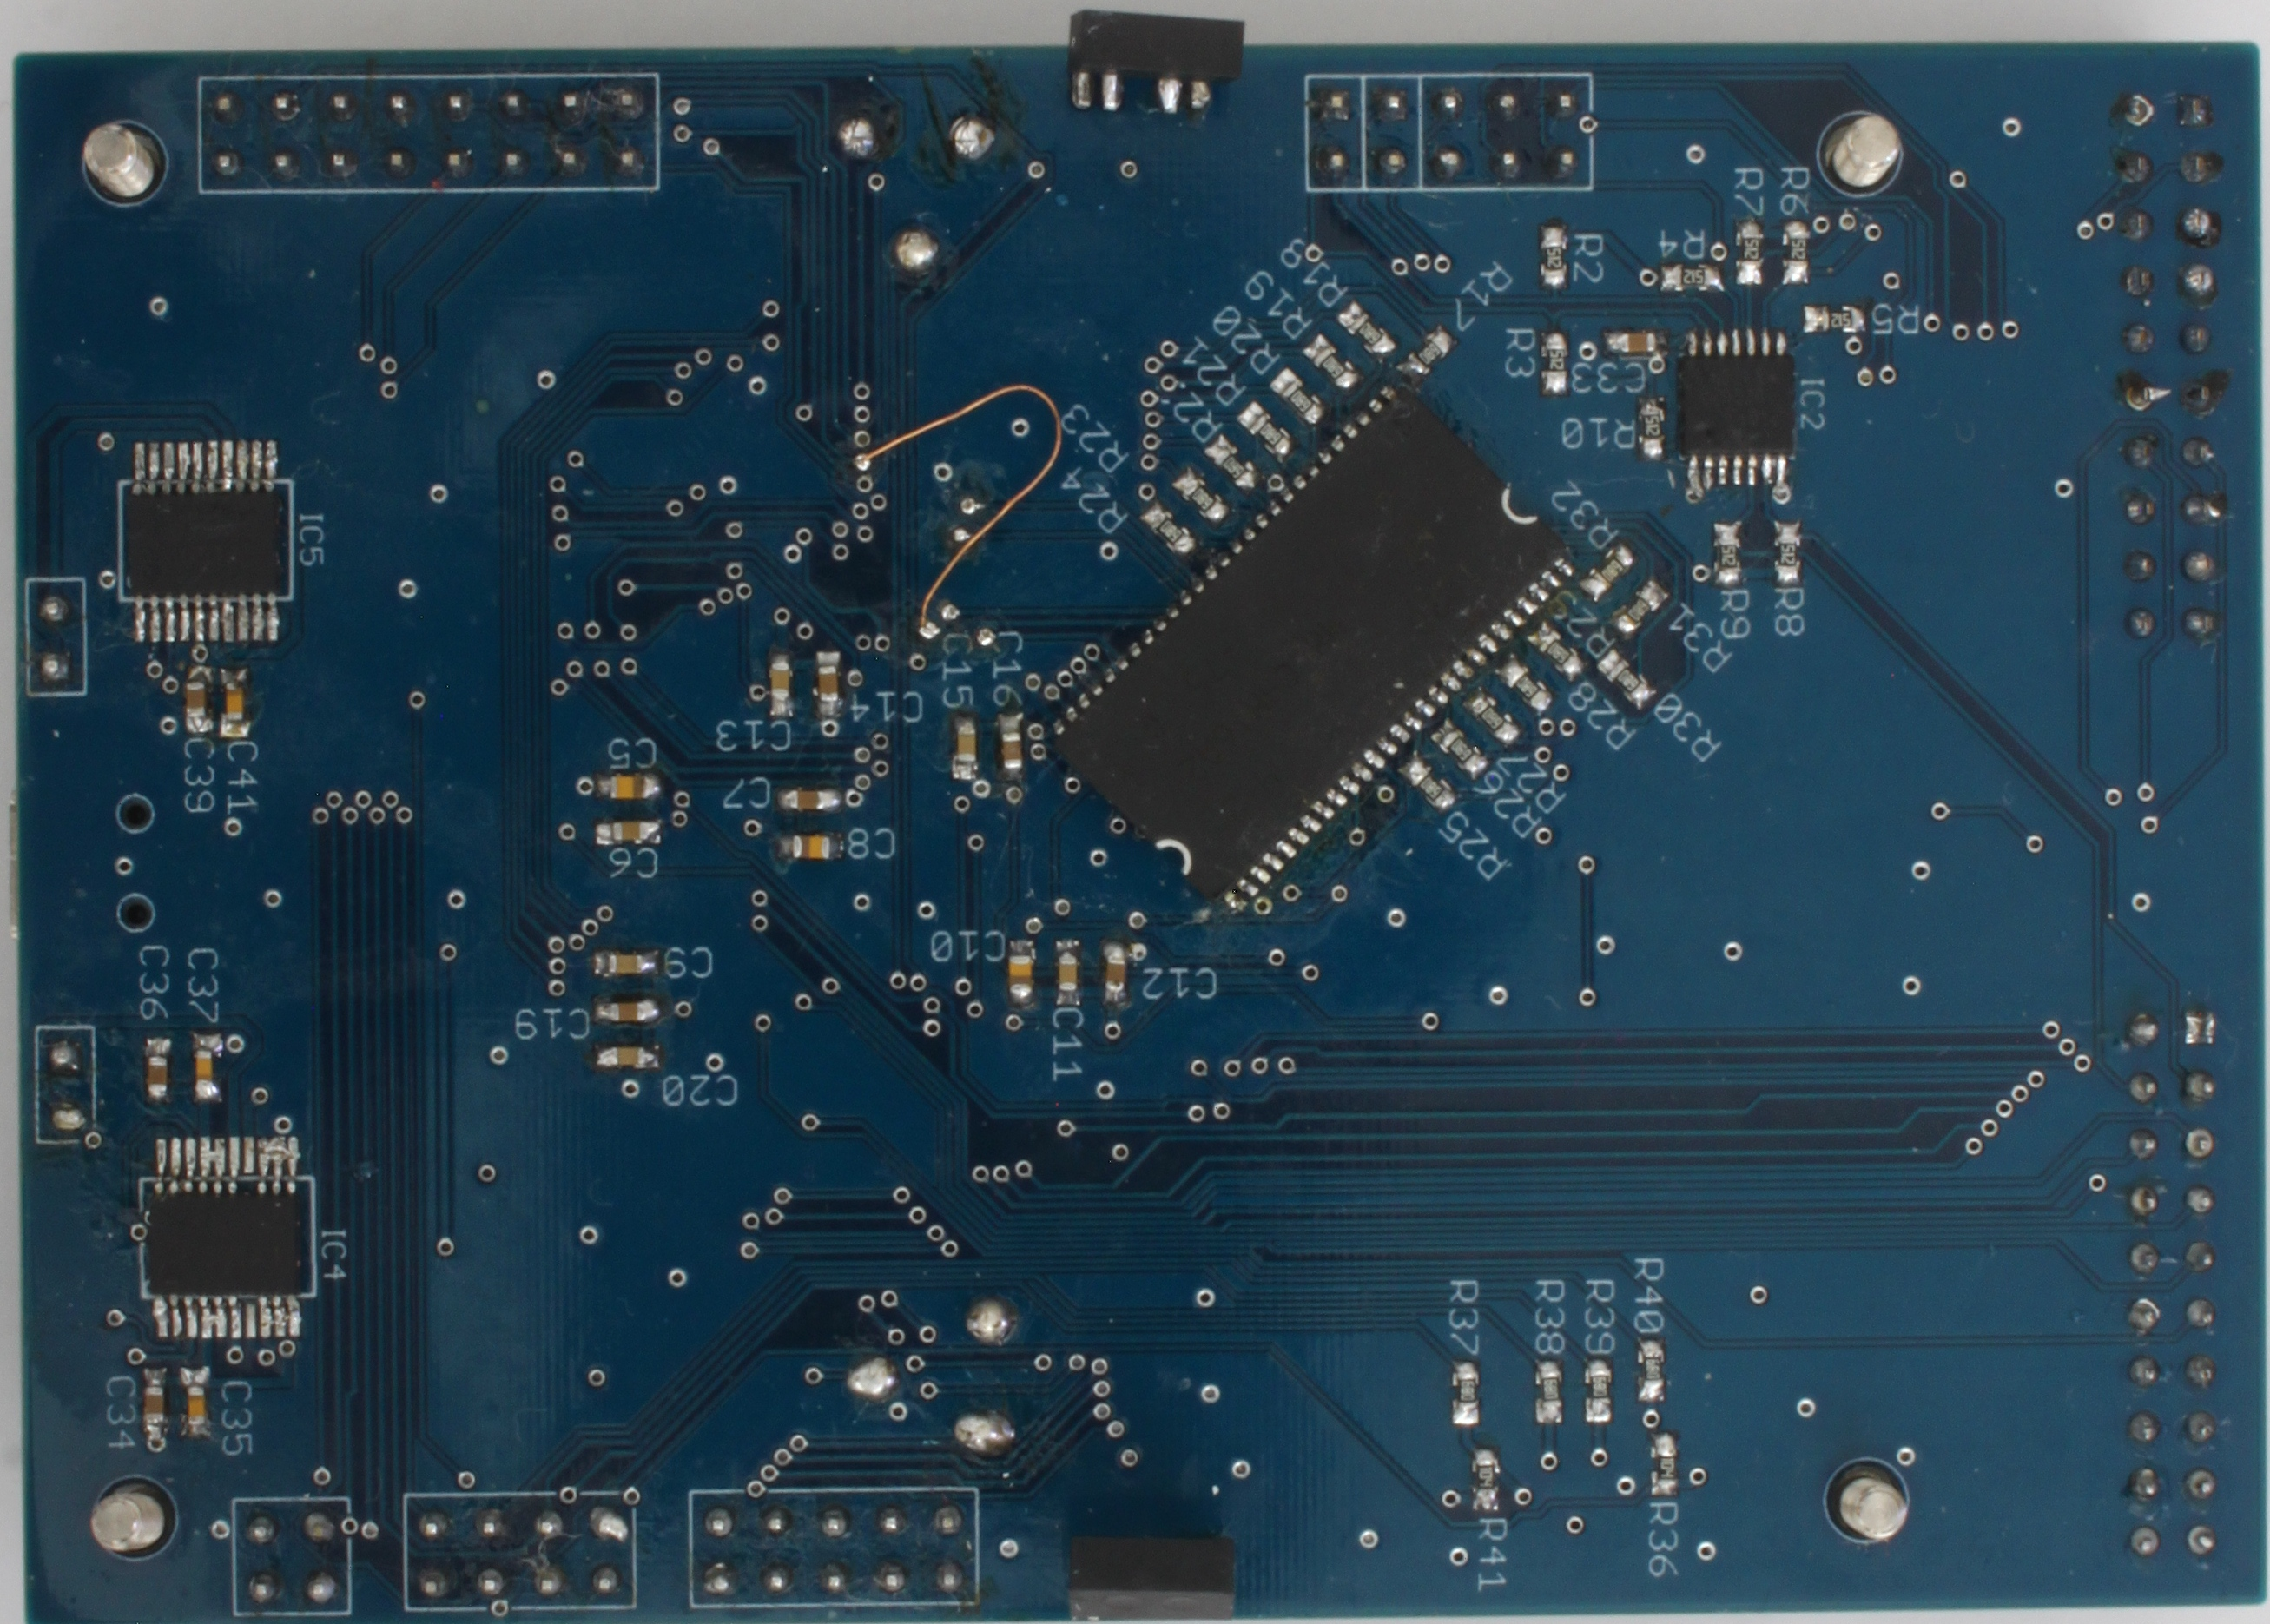
\includegraphics[width = \textwidth, keepaspectratio]{./Figures/PCB_Bottom.jpg} }
\caption{Pictures of the built PCB.}
\label{fig:PCB:Built}
\end{figure}
\section{Conclusions}

Overall, the hardware design and firmware is a success. A few minor faults were apparent on the PCB, but these were easily patched and caused no problems. Using a firmware test, the components are seen to be fully functional giving the UC3C full ability to control motors, cameras, \itc multiplexer, memory of both SD card (up to 2GB size) and external 4MB RAM. This provides a good platform for a manoeuvrable, stereoscopic vision robot to be developed. 